\documentclass[12pt]{article}   %  [titlepage]   \and
\usepackage{amsmath}
\usepackage[utf8]{inputenc}
\usepackage[T1]{fontenc}
\usepackage[danish]{babel}
\renewcommand{\rmdefault}{ptm}
\usepackage[pdftex]{graphicx}
\usepackage{multirow}
\newcommand{\nextitem}{\par\hspace*{\labelsep}\textbullet\hspace*{\labelsep}}
\usepackage{enumitem}
\usepackage{float}

\title{Kalender \& booking til K. Translation}
\author{Morten Trolle Nielsen - [14-06-79]\\ 
Øvrige deltagere i projektgruppen:\\
Omar Khalidan - [26-10-87]\\
    Instruktor: Andreas Frisch\\ \\
Projektkursus i Systemudvikling 2014 }

\begin{document}
\maketitle
\thispagestyle{empty}
\newpage
\tableofcontents
\newpage

\section{Abstract}
Dette er fjerde delrapport i faget Systemudvikling. Vi vil fortsætte arbejdet med og præsentationen af den IT-løsning, som vi er ved at udvikle til kunden; tolkeservicen K. Translation. Vores udgangspunkt er første, anden og tredie delrapport, som vi har udviklet og udbygget. Vi har analyseret anvendelsesområdet, skrevet de vigtigste use cases og på den baggrund opstillet de funktionelle og ikke-funktionelle krav. Udfra dette arbejde har vi modelleret problemområdet. Vi har også lagt os fast på en softwarearkitektur, og brugergrænsefladen er blevet afprøvet ved hjælp af den første prototype og mock-ups.  \\
Vi vil afslutte denne fjerde delrapport med to korte referater og efterfølgende analyse samt perspektivering af de to artikler, der er et krav til rapporten. Vi er selv førsteårs datalogistuderende ved Københavns Universitet, og det forventes, at læseren befinder sig på samme læringsniveau eller højere, idet der undervejs vil forekomme adskillige fagspecifikke termer. 

\newpage
\section{IT-projektet}
\subsection{It-projektets formål og rammer}

Tolkeservicen K. Translation (KT) er et lille tolkebureau med speciale i arabiske sprog. Indehaveren af bureauet er Souzane Khalidan, og hun er både leder og eneste medarbejder i bureauet. Hendes kunder er offentlige myndigheder såsom politiet, anklagemyndigheden og diverse ministerier, samt private aktører såsom advokatbureauer. Formålet med projektet er at udvikle et kalendersystem til KT, så KT's kunder nemt og hurtigt kan booke en aftale hos tolkeservicen, og rammerne indenfor hvilke, det skal foregå, er den teori og de metoder, vi er blevet præsenteret for i løbet af projektkurset. \\
\indent Udover at kalenderen vil gøre det nemmere for kunder og samarbejdspartnere at booke en aftale hos KT, så vil Souzane i hendes daglige, travle arbejde få stor gavn af en kalender, hvor alle aftaler er samlet et sted, eftersom hun idag må arbejde med tre eller fire forskellige kalendere. 


\subsubsection{Systemdefinition}
\indent Kalendersystemet vil bestå af et administrativ interface til brugeroprettelse, så Souzane selv kan tilføje nye kunder til systemet, og en hjemmeside med en kalender, som hendes kunder kan logge på, når de skal oprette en aftale. Derudover skal der sendes en bekræftende e-mail til kunden og en påmindelse til Souzane, hver gang en kunde opretter eller aflyser en aftale. Kundekartoteket placeres i en database, og alle indgåede aftaler placeres ligeledes i en database. \\  
\indent De efterfølgende FACTOR kriterier vil understøtte systemdefinitionen:\\

\begin{itemize}[noitemsep,nolistsep]
\item Functionality: Kalenderfunktion med mulighed for aftalebooking. Brugeroprettelse.

\item Application domain: Tolk. Kunder (oftest ministerielt ansatte, politi og lignende). Normalt kontormiljø. Systemadministrator. 

\item Conditions: Betjenes af kontorpersonale, der må forventes at bruge diverse kalendersystemer i deres daglige arbejde. Udvikles af datalogistuderende på baggrund af den fastlagte kravspecifikation. 

\item Technology: Udvikles på en billig PC med en udviklingserver og standardværktøjer. Det færdige system placeres hos en privat udbyder af serverplads til en fast månedlig pris.

\item Objects: Kalender og aftaler. Påmindelse og bekræftigelse. Kunde og kundekartotek. 

\item Responsibility: Planlægningsværktøj og kommunikationsmedium. 

\end{itemize}

\subsection{Use cases}
\indent Vi har bl.a. på baggrund af foredraget \emph{"Adgangs- og sikkerhedssystem til Københavns Lufthavne"} af Claus M. Andersen fra seminarrækken \emph{"IT der VIRKER"} valgt at placere vores use cases før kravspecifikationen og de funktionelle samt non-funktionelle krav. Claus Andersen beskrev, hvordan han og hans projektgruppe udarbejdede omkring 100 use cases, der efterfølgende kom til at danne grundlaget for kravspecifikationen. Vi vil følge dette eksempel og bruge vores use cases, når vi skal forhandle kravspecifikationen på plads med Souzane. Vi håber, at vi på den måde sammen og med en fælles forståelse for systemfunktionaliteten kan udarbejde en kravspecifikation, der er komplet og robust nok til, at der kommer så få ændringer som muligt i det videre projektforløb. (Vi har netop valgt et agilt projektforløb for at kunne tage højde for sådanne ændringer. Se evt. afsnittet om projektplan.)\\
\indent Figur \ref{fig:use} er et højniveau-diagram over samtlige use cases.

\begin{figure}[!ht]
\begin{center}
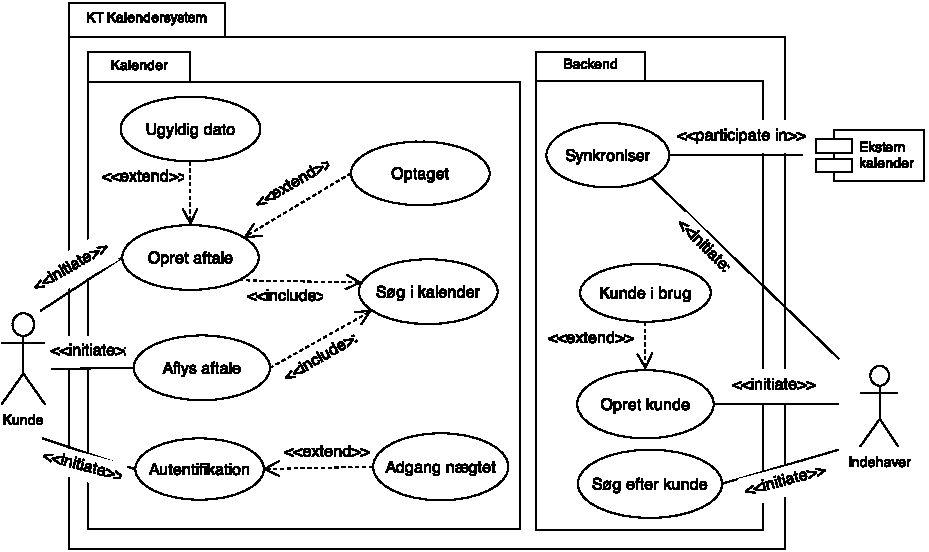
\includegraphics[width=14cm, height=7cm]{highlevel.pdf}
\caption{Højniveau use case diagram bestående af samtlige identificerede use cases.}
\label{fig:use}
\end{center}
\end{figure}
 
\indent Aktørerne i højniveau use case diagrammet er alle hentede fra anvendelsesområdet (application domain i FACTOR kriterierne). Indehaveren af KT er i dette scenario også systemadministrator, idet hun selv vil
skulle udfylde denne rolle på længere sigt. Hvis to use cases indeholder det samme begrænsede handlingsforløb, har vi modelleret dette med et ``include'' forhold. F.eks. kan en potentiel kunde søge i kalenderen, både når vedkommende opretter en aftale, og når vedkommende aflyser en aftale. Dette er med til at nedsætte kompleksiteten i use case modellen og fjerne redundans. Det samme gør sig gældende med ``extend'' forholdene, der modellerer undtagelser og fejltilstande som f.eks. systemets reaktion på ulovlige datoer eller mislykket login.\\
\indent Vi har valgt de 3 vigtigste use cases ud, og den første use case ``Opret kunde'' kan ses i tabel 1.\\

\hskip-1.0cm\begin{tabular}{l p{11cm}}
Use case navn & Opret kunde \\ \hline
Deltagere & \nextitem Initieret af KT's indehaver -
             Kommunikerer med kunde \\ \hline
Handlingsforløb &
	\nextitem Indehaveren af KT logger på systemet som administrator. 
	\nextitem  Administratorinterfacet viser menuen.
	\nextitem Indehaveren navigerer til menupunktet, hvor man kan tilføje nye	kunder.
		\nextitem Interfacet præsenterer en formular til indehaveren.
	\nextitem KT's indehaver udfylder samtlige formularfelter med kundens stamdata og anden kontaktinformation. Derefter sender hun formularen.		
	\nextitem Administratorinterfacet tilføjer kunden til kundekartoteket
	og autogenererer en e-mail, der sendes til den aktuelle kunde
		med besked om, at vedkommende nu kan logge på systemet for at
		booke en tid.
	\nextitem KT's indehaver logger af systemet. 
	\nextitem Interfacet lukkes.
	\\ \hline
	Indgangs betingelse &
		\nextitem KT's indehaver er logget på administratorinterfacet. 
		\nextitem Pågældende kunde er ikke oprettet i kundekartoteket. 
		\\ \hline
Exit betingelse & 
	\nextitem Pågældende kunde er nu tilføjet til
			kundekartoteket.
		\nextitem Der ligger en bekræftende e-mail i den pågældende kundes
			indbakke.
		\nextitem KT's indehaver er logget af systemet.\\ \hline
	\end{tabular}
\begin{center}
\textbf{Tabel 1}: I denne use case opretter KT's indehaver en kunde i kundedatabasen.
\end{center}
\vspace{0.5cm}

Denne use case beskriver, hvordan K. Translations indehaver opretter en ny kunde i kundedatabasen. Det er vigtigt, at Souzane selv på længere sigt kan overtage rollen som systemadministrator og tilføje nye kunder til databasen, så derfor er denne use case specielt vigtig. \\ 
\indent Den anden use case, vi har valgt, hedder ``Opret aftale''. Se tabel 2. \\

\hskip-1.0cm\begin{tabular}{l p{11cm}}
Use case navn & Opret aftale \\ \hline
Deltagere & \nextitem Initieret af KT's kunde
            - kommunikerer med KT's Indehaver\\ \hline
Handlingsforløb &
	\nextitem KT's kunde navigerer til KT's hjemmeside, hvor kunden logger
	på med det personlige password.
	\nextitem Kalenderkontrollen henter kalenderen og viser den til
	kunden.
	\nextitem Kunden vælger at oprette en aftale.
	\nextitem Kalenderkontrollen henter en formular, som kunden skal
	udfylde.
	\nextitem Kunden indtaster datoen og klokkeslettet for den ønskede 
	aftale og bekræfter.
	\nextitem Kontrollen validerer dato samt klokkeslet og præsenterer
	kunden for en menu med forskellige aftaletyper.
	\nextitem Kunden vælger den ønskede aftaletype og bekræfter.
	\nextitem Kontrollen opretter aftalen i kalenderen og sender
	automatisk en e-mail til både kunden og indehaveren af KT. 
	\nextitem Kunden logger af kalenderen.
	\\ \hline
	Indgangs betingelse &
		\nextitem KT's kunde er logget på kalenderen. 
		\nextitem Kalenderen indeholder ingen aftaler på det af kunden
		ønskede tidspunkt.
		\\ \hline
Exit betingelse & 
	\nextitem Der er oprettet en aftale i kalenderen på det ønskede
	tidspunkt. 
		\nextitem Der ligger en bekræftende email i den pågældende kundes
			indbakke.
		\nextitem Det ligger en e-mail i KT's indehavers
			indbakke med dato og tidspunkt for aftalen. 
		\nextitem Kunden er logget af systemet.\\ \hline
		Kvalitets krav & Da det er muligt for kunden at søge i kalenderen, kan denne use case på et vilkårligt tidspunkt inkludere use casen  ``Søg i kalender''. Hvis dette sker, kan kunden søge i kalenderen, enten ved at bladre frem èn dag eller uge	ad gangen eller ved at søge på en dato længere ude i fremtiden.\\ \hline
\end{tabular}
\begin{center}
\textbf{Tabel 2}: I denne use case opretter en kunde en aftale i kalenderen.
\end{center}
\vspace{0.5cm}

Her logger en kunde på systemet for at booke en aftale med tolkeservicen, og vedkommende skal både oplyse dato, klokkeslet og opgavetype. Dette er en helt central funktion og selve berettigelsen for kalendersystemet, så derfor er denne use case medtaget.\\
Efter at have vist to almindelige use cases, har vi til sidst valgt at fokusere på de særlige forhold, der gør sig gældende ved en ``extend'' use case ved at præsentere use casen ``Ugyldig dato''. Se tabel 3. Konteksten for denne use case er ``Opret aftale'' use casen fra tabel 2, som på et givent tidspunkt i handlingsforløbet, hvis kunden indtaster en ugyldig dato, vil blive udvidet med ``Opret aftale'' use casen. \\

\hskip-1.0cm\begin{tabular}{l p{11cm}}
Use case navn & Ugyldig dato \\ \hline
Deltagere & \nextitem Kommunikerer med KT's kunde.
            \\ \hline
Handlingsforløb &
	\nextitem Kunden oplyser kontrollen om, at vedkommende vil oprette en
	aftale.
	\nextitem Kontrollen opretter en formular til aftalen.
	\nextitem Kunden indtaster dato og klokkeslet for aftalen og
	bekræfter.
	\nextitem Formularen prøver at validere tidspunktet, men den fejler.
	Kontrollen beder kunden indtaste et nyt tidspunkt.
	\nextitem Kunden indtaster dato og klokkeslet for den nye aftale og
	bekræfter.
	\nextitem Formularen prøver at validere tidspunktet og godkender.
	Kontrollen spørger kunden om opgavetypen.
	\nextitem Kunden oplyser opgavetypen og bekræfter.
	\\ \hline
	Indgangs betingelse &
		\nextitem Denne use case udvider ``Opret aftale'' samt ``Aflys
		aftale'' use cases. Den initieres, når formularen ikke kan
		validere tidspunktet for kundens aftale, fordi kunden har
		indtastet et ikke eksisterende tidspunkt.  
		\\ \hline
Exit betingelse & Der ligger en gyldig aftale i kalenderen på en lovlig dato.
	\\ \hline
\end{tabular}
\vspace{0.3cm}

\textbf{Tabel 3}: Denne <<extend>> use case ``Ugyldig dato'' udvider den forrige use \\ \indent case, hvis en bruger indtaster en ugyldig dato.        

\vspace{0.5cm}

Dette var de tre vigtigste use cases. Desværre havde vi ikke mulighed for at involvere slutbrugerne fra anvendelsesområdet i arbejdet med disse use cases, hvilket  ville have været at foretrække, eftersom disse personer ligger inde med en værdifuld viden om problemområdet og arbejdsgange (både hensigtsmæssige og uhensigtsmæssige), og fordi deres erfaringer med den tidligere måde at gøre tingene på kombineret med deres ønsker til den nye måde kun ville øge værdien af vores use cases.

\subsection{Kravspecifikation}

Før vi fortsætter med modelleringen af problemområdet, vil vi præcist beskrive, hvilke krav og forventninger kunden, K. Translation, har til vores endelige løsning. Kravspecifikationen er blevet til på baggrund af vores kundemøder, kundens krav og forventninger og vores udarbejdede use cases og består af følgende tre dele: de funktionelle og non-funktionelle krav samt constraints. Idet kravspecifikationen senere kommer til at ligge
til grund for afprøvningen og test af systemet, er det vigtigt, at den er ``komplet, konsistent, entydig og korrekt.''\cite{oose}[p.~122] \\

\subsubsection{Funktionelle krav}

\rule{120mm}{1mm}
\begin{itemize}
\item KT's kunder skal på hjemmesiden præsenteres for en login menu, hvor de logger på systemet med et brugernavn og et password.
\item It-løsningen skal indeholde en kalender med ledige og optagede tidspunkter.
\item Der skal være et tilhørende bookingsystem, så kunderne kan lave en aftale med KT.  
\item Det skal være muligt for kunderne at søge i kalenderen efter ledige tidspunkter.
\item KT's kunder skal kunne vælge mellem mundtligt eller skriftligt tolkearbejde.
\item Der skal sendes en bekræftende e-mail tilbage til kunden, efter at vedkommende har booket en tid i kalenderen. 
\item KT modtager ligeledes en e-mail med dato, klokkeslet, kunde og opgavetype.
\item Det skal være mulig for kunderne at aflyse en aftale.
\item Det skal være muligt for KT løbende at tilføje flere kunder eller samarbejdspartnere til databasen. 
\item KT's indehaver vil gerne kunne overføre sine private aftaler fra en ekstern kalender til vores kalendersystem. Hun forestiller sig en form for synkronisering, men vi har fra start gjort hende det klart, at dette måske for os er en for kompliceret opgave. 
\end{itemize}
\rule{120mm}{1mm}
\vspace{0.5cm}

\subsubsection{Non-funktionelle krav}

\rule{120mm}{1mm}
\begin{itemize}
\item Designet skal være enkelt	og intuitivt, så personer uden store it-forudsætninger kan navigere på siden og booke en tid inden for 2 min.
\item Indehaveren vil have et system, der ikke kræver løbende	vedligeholdelse, men som bare ``kører og passer sig selv''.   
\item Der ønskes præcis og let forståelig dokumentation af systemet. 
\item Kalendersystemet og backend databasen må ikke tabe data eller aftaler, da dette betyder tabt indkomst for KT.
\end{itemize}

\rule{120mm}{1mm}
\vspace{0.5cm}

Da belastningen af systemet ikke forventes at blive særlig høj, har KT ingen performancemæssige krav til vores løsning. Der er ingen tidskritiske brugerfunktioner, og risikoen for samtidig brug af kalenderen må forventes at være minimal. Hvis to kunder vil booke den samme 
tid i kalenderen, og dette medfører en race condition, burde backend databasens transaktionsindstillinger kunne håndtere dette.\\


\subsubsection{Constraints}
\rule{120mm}{1mm}
\begin{itemize}
\item KT ønsker en it-løsning, som af bureauets kunder kan tilgås over internettet via en hjemmeside.
\item Alle brugere skal kunne tilgå systemet med en almindelig web browser som Internet Explorer, Firefox eller Google Chrome.
\item Hjemmesiden skal indeholde KT's kontaktinformationer.
\item KT ønsker, at vi selv står for installationen af det færdige system.
\item KT ønsker den letteste og billigste implementering og hosting af systemet.
\end{itemize}
\rule{120mm}{1mm}\\

Vi synes, at kravspecifikationen på en god og dækkende måde beskriver de ønsker, som KT har til det færdige program. Eftersom der ikke var noget legacy kalendersystem, som vi kunne læne os op ad, brugte vi i stedet for vores use cases som udgangspunkt for kravspecifikationen. Selvom flere af de non-funktionelle krav er svært verificerbare (hvornår er noget enkelt, intuitivt og letforståelig ?), så burde det være muligt at teste, om vores løsning lever op til de ovenstående krav, når systemet senere skal valideres på baggrund af kravspecifikationen.  

\subsection{Problemområdet}

Vi kan nu på baggrund af vores use cases og kravspecifikationen gå i gang med at modellere problemområdet. Vi præsenterer for overskuelighedens skyld først et UML-diagram over området, se figur \ref{fig:problem} på næste side, og dernæst følger en liste over de klasser, vi har modelleret i problemområdet.

\begin{figure}[!ht]
\begin{center}
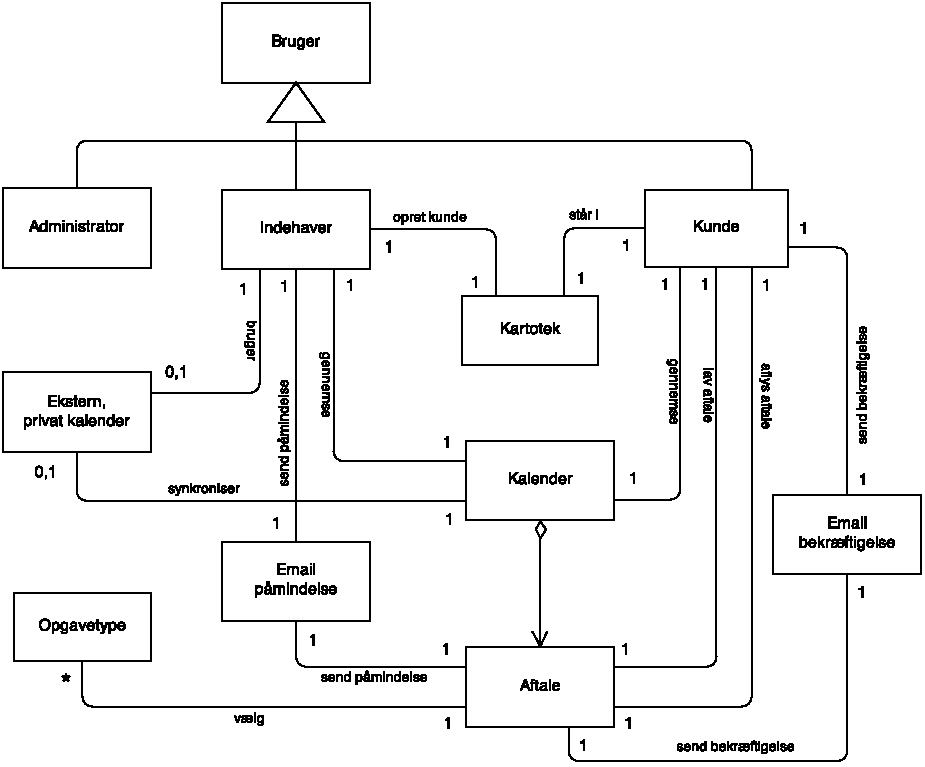
\includegraphics[width=12cm, height=12cm]{problemomr.pdf}
\caption{UML-diagram over problemområdet.}
\label{fig:problem}
\end{center}
\end{figure}

\begin{itemize}
\item Bruger: Kunde, administrator, indehaver. Går igen fra
	anvendelsesområdet.
\item Et kundekartotek, hvor KT's indehaver løbende kan tilføje kunder.
\item Kalenderen, som kunderne kan bruge, når de skal finde en ledig tid, og som KT's indehaver kan bruge i sit daglige, travle arbejde.
\item Aftale. Kunderne booker en aftale i kalenderen.
\item Da KT har både mundtlige, skriftlige og andre opgaver, skal kunden	oplyse typen på arbejdet.
\item Kunden får en bekræftende e-mail tilsendt med det aftalte tidspunkt.
\item KT's indehaver får ligeledes en påmindelse tilsendt pr. e-mail, når der er oprettet en aftale i kalenderen. 
\item KT's indehaver har et ønske om at kunne synkronisere hendes eksterne, private kalender med vores it-løsning.
\end{itemize}

Det første, vi har modelleret, er brugerne fra anvendelsesområdet, idet disse skal have adgang til klasserne i problemområdet. Souzane skal kunne oprette nye kunder i kundekartoteket, og eksisterende kunder står opførte i dette kartotek. Endvidere skal Souzane kunne tilgå kalenderen for at tjekke aftaler og evt. selv lægge nye aftaler ind. Kunderne selv vil efter login have adgang til kalenderen, hvor de kan søge efter ledige tidspunkter og oprette aftaler. Kalenderen kan indeholde mange aftaler, og derfor er relationen mellem disse to klasser modelleret med aggregering. Når kunden har oprettet eller aflyst en aftale, sendes der automatisk en bekræftende e-mail til kunden og en påmindelse til KT. \\
Vi har også modelleret synkroniseringen af Souzanes eksterne, private kalender med vores kalendersystem, så hun kan overføre private aftaler og samle dem alle i en kalender. (Hvis denne opgave viser sig for kompliceret, må Souzane manuelt indtaste sine private aftaler i vores kalender.) \\
\indent Hermed slutter gennemgangen af problemområdet. Den ovenstående modellering vil ligge til grund for det videre design og endelige system. 

\subsection{Sekvensdiagrammer}

På baggrund af de tidligere gennemgåede use cases, har vi tegnet 3 sekvensdiagrammer. Vi vil i vores gennemgang fokusere på at identificere entitet-, grænseflade- og kontrolobjekterne.\footnote{De engelske betegnelser er henholdsvis entity-, boundary- og control objects, men vi har valgt at beholde de danske betegnelser.} Sekvensdiagrammet over første use case ``Opret kunde'' kan ses i figur \ref{fig:opret}. \\

\begin{figure}[!ht]
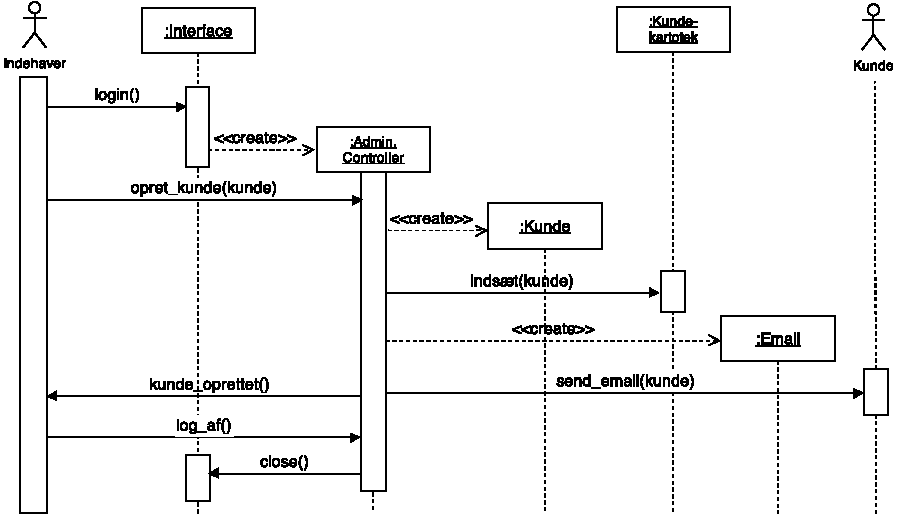
\includegraphics[width=14cm, height=10cm]{seqtwo.pdf}
\caption{Sekvensdiagram over første use case ``Opret kunde''.}
\label{fig:opret}
\end{figure}

Grænsefladeobjekterne er administratorinterfacet, hvorfra indehaveren logger på systemet, og formularen, hvor vedkommende indtaster kundens stamdata. Den bekræftende
e-mail er også en del af grænsefladen, selvom den ikke går til indehaveren men til kunden. Kundekartoteket er den ene entitet, og kunde er den anden. (Her tænker vi ikke på kunden som aktør, men som en entitet der oprettes undervejs
udfra de indtastede stamdata). Administratorkontrollen er ansvarlig for at oprette entiteten kunde og grænsefladerne e-mail samt aftaleformular. \\
\indent Det andet sekvensdiagram er over use casen ``Opret aftale''. Se figur \ref{fig:aft}. \\

\begin{figure}[!ht]
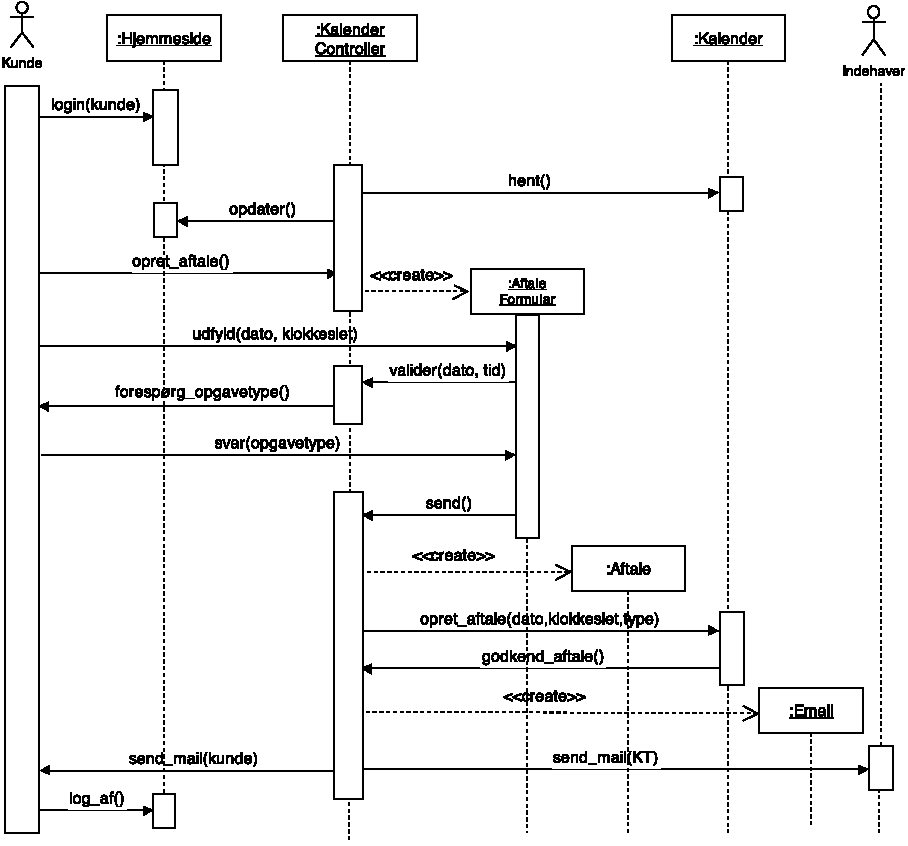
\includegraphics[width=14cm, height=11cm]{seq.pdf}
\caption{Sekvensdiagram over use casen ``Opret aftale''.}
\label{fig:aft}
\end{figure}

Grænsefladeobjekterne er KT's hjemmeside, hvorfra der logges på systemet, og formularerne, der udfyldes af kunden undervejs samt de to afsendte e-mails. Kalenderen og aftalen er entiteter, og kalenderkontrollen er kontrolobjektet. \\
\indent Det sidste sekvensdiagram viser extend use casen ``Ugyldig dato''. Se figur \ref{fig:extseq}. Grænseflade-, kontrol- og entitetobjekterne vil være magen til objekterne i den use case eller det sekvensdiagram, hvori undtagelsen indtræffer.

\begin{figure}[!ht]
\begin{center}
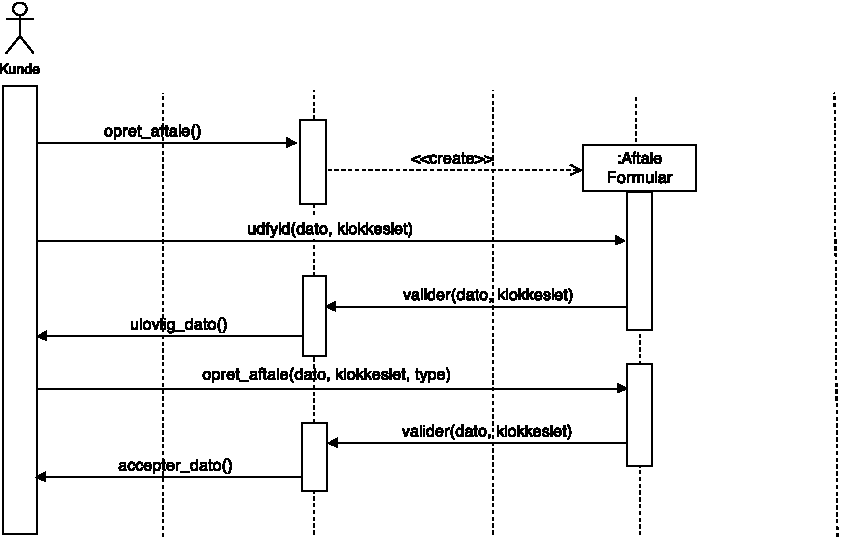
\includegraphics[width=14cm, height=11cm]{extend.pdf}
\caption{Sekvensdiagram for ``Optaget'' samt  ``Ulovlig dato''.}
\label{fig:extseq}
\end{center}
\end{figure}

Vi har valgt at identificere grænseflade-, kontrol- og entitetobjekter på nuværende tidspunkt, så dette arbejde bl.a. kan ligge til grund for det næste afsnit om softwarearkitektur og designmønster. 

\section{Systemdesign}

Vi har valgt at implementere systemet med det Model-View-Controller (MVC) baserede webframework Django.  En af Djangos helt store styrker, som udspringer af MVC arkitekturen, er den løse kobling og strenge adskillelse mellem de forskellige dele af modellen. Det betyder, at vi let kan ændre, slette eller tilføje i eksisterende dele uden at bekymre os om afhængigheder mellem delene.\\ \indent Derudover har vi valgt en client-server løsning, hvor brugerne tilgår kalenderen, der er placeret på serveren, via deres egen browser. Se figur \ref{fig:mvc}. Client-server løsningen opfylder lige præcis vores behov, og havde vi valgt en anden evt. multilagdelt arkitektur, havde vi ikke vundet andet end øget kompleksitet.

\begin{figure}[!ht]
	\centering
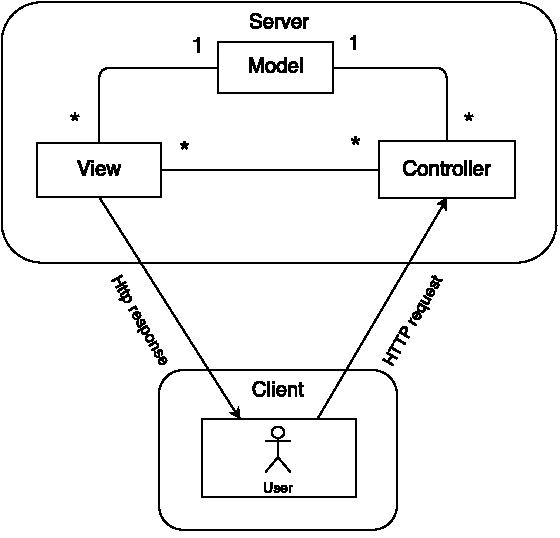
\includegraphics[width=9cm, height=8cm]{mvc.pdf}
\caption{Model-View-Controller arkitektur superimposeret på client-server.}
\label{fig:mvc}
\end{figure}

Valget af Django skal også ses i forhold til vores arbejde med use cases og sekvensdiagrammer. Vi fokuserede på at identificere entiteterne, grænsefladerne samt kontrollerne, og disse objekter kan vi nu kortlægge til model, view og controller\footnote{Model svarer til entitet, view til grænseflade og controller til kontrol.}. Vores model kommer til at bestå af de aftaler, som KT's kunder booker ind i kalenderen. Django's templates står for præsentationen og grænsefladen, og vi påtænker at bruge en basisskabelon til hjemmesiden, der udvides med tilpassede templates, når logikken kræver det. Selve forretningslogikken bliver implementeret i Django's viewfunktioner. (Controller i MVC). Det er bindeleddet mellem modellen og grænsefladen, og det er her, kernefunktionaliteten kommer til at sidde.\\ 

\section{Brugergrænseflade og interaktionsdesign}
\subsubsection{Flowcharts og mock-ups}

Vi præsenterer her den første prototype af systemet i form af mock-ups af det påtænkte design. Derudover tegner vi de vigtigste flowcharts, så vi kan få et overblik over dynamikken i systemet. Vi vil få en person, der ikke er tilknyttet projektet, til at gennemgå vores prototype mock-up. Det mest ideelle ville dog have været, at få en virkelig bruger af det endelige kalendersystem, til at evaluere prototypen, men det har ikke været muligt på nuværende tidspunkt.
Det første flowchart viser dynamikken i systemet fra en bruger logger på til vedkommende logger af. Se figur \ref{fig:flow1}.\\

\begin{figure}[!ht]
\begin{center}
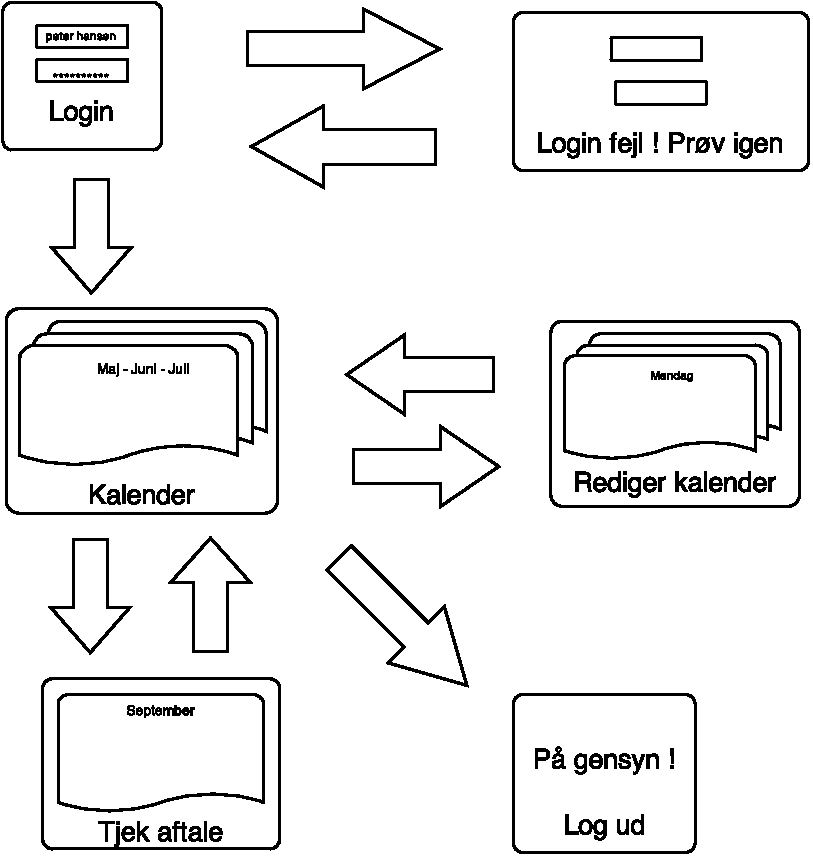
\includegraphics[width=8cm, height=8cm]{flow1.pdf}
\caption{Flowchart over kalendersystemet}
\label{fig:flow1}
\end{center}
\end{figure}

Brugeren vil efter succesfuldt login blive dirigeret videre til en side, der viser den aktuelle måned. Det skal være muligt for brugeren at trykke sig fremad månedsvis, så vedkommende kan indsætte en aftale i kalenderen uger eller måneder ude i fremtiden, men det skal ikke være muligt at bladre tilbage i kalenderen, eftersom dette ikke vil bibringe kalenderen nogen merværdi. Brugeren kan nu vælge mellem to veje: enten at tjekke kalenderen igennem uden at oprette eller aflyse nogen aftaler, eller vedkommende kan vælge at redigere i kalenderen. Vi har tegnet et nyt flowchart, der viser forløbet, hvis brugeren vælger at redigere i kalenderen. Se venstre side af figur \ref{fig:flow2}. Dette udvikler det første overordnede flowchart, og vi har bl.a. brugt sekvensdiagrammerne samt de relevante use cases fra afsnit 4 til at udvikle brugergrænsefladen, så der er overensstemmelse mellem de forskellige designfaser. \\


\begin{table}[ht]
\centering
\begin{tabular}{l | r}
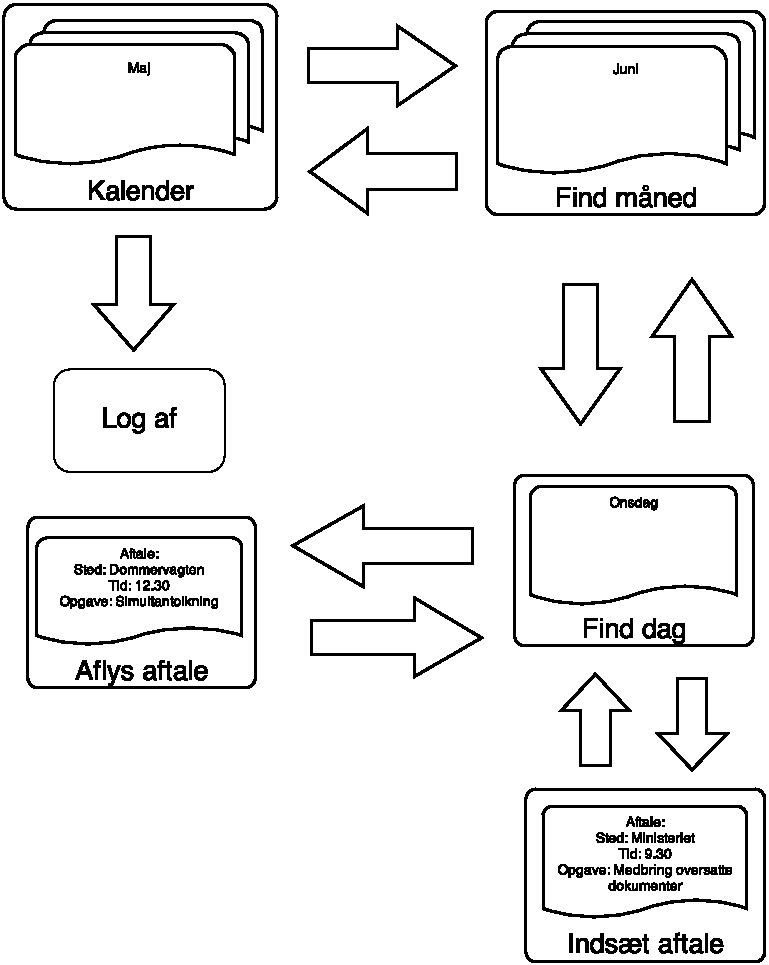
\includegraphics[height=7cm,width=7cm]{flow2.pdf}
\label{fig:flow2}&
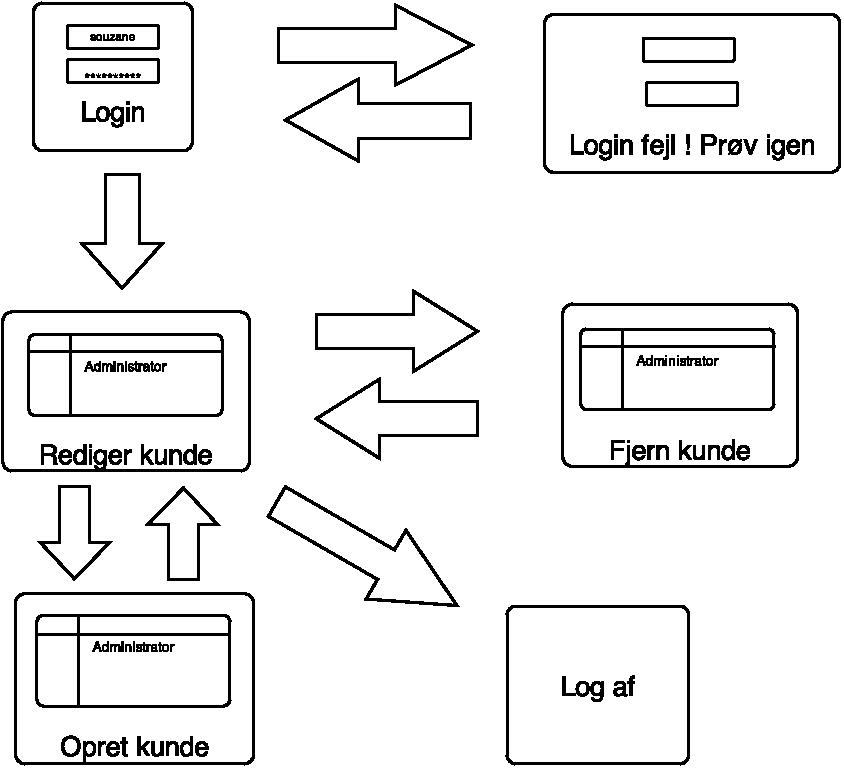
\includegraphics[height=7cm, width=7cm]{flow3.pdf}
\\
\end{tabular}
\label{tab:gt}
\end{table}
\begin{centering} \textbf{Figur \ref{fig:flow2} og 8.2 :} To flow-charts. Det venstre viser navigation i kalenderen samt oprettelse og aflysning af aftale. Det højre viser oprettelsen af en kunde. 
\end{centering}

\vspace{0.5cm}

Flowchartet viser de to veje, man kan følge, hvis man enten skal aflyse eller oprette en aftale. Højre side af figur \ref{fig:flow2} viser forløbet, hvis Souzane enten skal oprette eller fjerne en kunde i systemet. Vi vil ikke gøre mere ud af disse flowcharts, men i stedet for gå videre til den prototype af kalenderen, vi har designet i form af mock-ups. \\

\subsection{Prototype, mock-ups og tænke-højt-forsøg}
Vi har nu lagt os fast på et design af kalenderen, og vil gerne have det testet af en bruger, inden vi begynder at kortlægge modellen til kode. Derfor har vi lavet en mock-up model af kalendersystemet bestående af 5 tegninger, der, når de vises i den rigtige rækkefølge, kan gøre det ud for et normalt handlingsforløb, som det vi så i use casen "Opret aftale" fra afsnit 4, og som det også fremgik af forrige flowcharts. \\
Alle fem mock-up tegninger kan ses i korrekt rækkefølge i bilag 1, men de er grundet pladshensyn ikke taget med her. Vi har som sagt ikke testet mock-up'en på en rigtig end-user, men har fået vores kammerater, der alle selv er igang med lignende projektforløb, til at teste modellen ved et tænke-højt-forsøg. Det betyder, at vi får svært ved at sætte kalenderen ind i en rigtig kontekst, da vi ikke kan simulere en travl arbejdsdag med telefoner, der ringer, og møder, der skal nås. Til gengæld håber vi på, at fordi vores kammerater selv er igang med lignende projekter, så har de en nysgerrig og professionel tilgang til opgaven. \\
Testen forløb på den måde, at en testperson blev stillet en opgave, der lød: Book en aftale i kalenderen. Derefter blev personen præsenteret for den første tegning med en login menu, og når vedkommende havde udfyldt denne korrekt, så fik personen næste tegning fremlagt. Dette fortsatte indtil, at der var oprettet en aftale i kalenderen, og testpersonen havde modtaget en bekræftigelse på aftalen. Mens vi præsenterede personen for tegningerne, overvågede Omar og jeg forløbet, og vi lagde mærke til, hvor testpersonen havde let ved at forstå designet, og hvor der var misforståelser og forvirring. Vi måtte ikke kommunikere med testpersonen undervejs, medmindre vedkommende sad fuldstændig fast, men udelukkende lytte til hvilke overvejelser, testpersonen gjorde sig undervejs. Bagefter evaluerede vi forsøget med testpersonen. Her har vi samlet nogle af de hyppigste bemærkninger:

\begin{itemize}
\item Enkelt og simpelt design.
\item De var en, der mente, at det måske var for simpelt. Vedkommende kunne godt tænke sig nogle flere funktioner som f.eks. en hjælpe- / supportfunktion.
\item Der var lidt forvirring om, hvordan man kom fra månedskalenderen til dags dato-visningen. Nogle troede, at pilen til at navigere frem i kalenderen ville føre dem til den valgte dag. 
\item Ellers blev månedskalenderen opfattet som overskuelig og nem at gå til. 
\item Der var nogen forvirring omkring, hvordan man lægger en aftale ind under dags dato.
\item Der var flere, der begyndte at indsætte aftalen allerede på mock-up tegning 3. 
\item Det var ikke helt klart for testpersonerne, hvordan de skulle booke en aftale, hvor tidsintervallet måske var 4 timer. De forsøgte enten at skrive aftalen ind hver halve time, eller at markere et større tidsinterval med musen.
\item Der var nogle, der mente, at det krævede for mange videre-klik af booke en aftale, og at der var for mange forskellige skærmbilleder undervejs i forløbet. De syntes, at vi skulle overveje at forenkle designet. Folk, der logger ind på kalenderen, ved som regel præcist, hvornår de vil booke en aftale, og for dem vil det være et irritationsmoment at skulle igennem flere irrelevante skærmbilleder. 
\item Der var også flere, der påpegede, at for folk der ofte bruger kalenderen, vil det ikke være optimalt, at de hver gang skal udfylde de samme oplysninger. Disse oplysninger kunne godt være indsat på forhånd.
\end{itemize}

Som det fremgår, kom vores testpersoner med mange gode observationer og ideer til designet. Vores egen største udfordring indtil videre har også været, hvordan man lettest og hurtigst kan indsætte en aftale i kalenderen. Hvis vi skal dømme efter testpersonerne, har vi måske ikke helt løst denne opgave endnu, og derfor må vi gennemgå visse aspekter af designet igen, inden vi koder flere fejl og uhensigtsmæssigheder ind i systemet. \\

\subsection{Audio-visuel præsentation af brugergrænsefladen}
Dette punkt planlægger vi at lave til sidst i forløbet, så vi har så meget som muligt at præsentere i videoen. 


\section{Projektplan}
Adskillige forelæsninger i Systemudviklingskurset har handlet om agil projektledelse og systemudvikling. Vi har fundet en sådan iterativ og inkremental tilgang til projektet spændende og kunne derfor godt tænke os at systemudvikle inden for rammerne af de agile principper, som vi bl.a. har 
stiftet bekendsskab med i artiklen ``Jeff Sutherland's Scrum
Handbook''\cite{scrum}. Det vil dog ikke være muligt, at gennemføre projektet i komplet overensstemmelse med Scrum og alle de agile regler. For det første vil det betyde, at vores kunde skal afse betydelig mere tid til projektet, end hun umiddelbart har planlagt, hvis hun løbende skal opdate ``Product Backlog'' og deltage i prioriteringsmøder ved hver sprints begyndelse. Derudover vil det ikke være realistisk, at vi selv holder daglige Scrum møder,
og at vi kan levere al den dokumentation et virkeligt Scrum forløb forudsætter som f.eks. de daglige overslag over vores egne fremskridt i forhold til opgaverne i den aktuelle sprint. Derfor vil vi slække på nogle af 
reglerne, og vi håber at kunne gøre det uden at bevæge os alt for langt væk fra den virkelige agile Scrum systemudvikling.\\
I stedet for de daglige estimeringer over projektets fremadskriden, har vi valgt at nøjes med et overordnet burndown diagram for hele projektet. Se figur
\ref{fig:bd}. (Et burndown diagram for en enkelt sprint vil være magen til, men værdierne på førsteaksen vil være dage i stedet for uger, og værdierne på
andenaksen vil være mindre). 

\begin{figure}[!ht]
	\centering
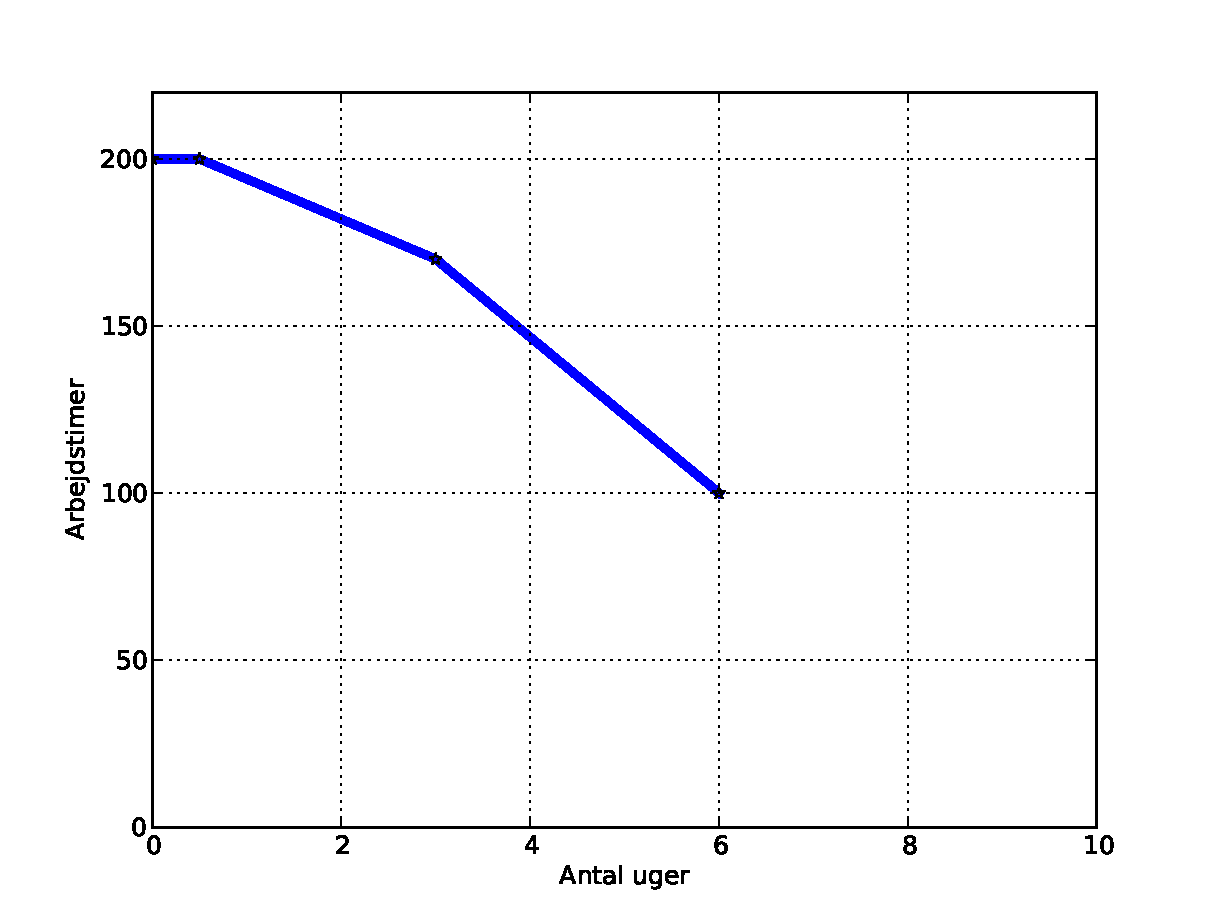
\includegraphics[width=13cm, height=9cm]{burn.pdf}
%\caption{Burndown diagram over projektforløbet}
\label{fig:bd}
\end{figure}
\begin{center}
\textbf{Figur 9:} Burndown diagram over projektforløbet
\end{center}

Vi har som udgangspunkt afsat mellem 8 og 10 uger til det agile projektforløb og bedømt den påkrævede arbejdsindsats til at være 200 timer, hvilket vil sige 100
timer til hver, da vi er to mand i gruppen. Dette overslag er dog yderst usikkert, men vi har aldrig prøvet at arbejde på denne måde før, så det bliver spændende at se, om vores estimationer bliver mere præcise undervejs. Vi har
planlagt at udvikle i sprints af 14 dages varighed, men vi kan udvide dette til 3 uger, hvis et af punkterne i produkt backloggen forekommer mere omfangsrigt.\\
Indehaveren af K. Translation har ofte meget travlt og kan som sagt ikke deltage i hvert nyt sprintmøde. Derfor har vi besluttet at simulere disse møder ved, at vi selv skriver og opdater produkt backloggen og gør det med udgangspunkt i kravspecifikationen. Vi bliver herved in effect vores egen 
proxykunde. Den anden produkt backlog kan ses i tabel 5. Den første produkt backlog kan ses i bilag B.

\begin{center}
	\begin{tabular}{|p{8cm}|l|l|l|}
		\hline
Punkt & Prioritet & Værdi & Timer \\ \hline
Som bruger af KT's hjemmeside bliver man præsenteret for en kalender, hvori man
kan booke en aftale med KT. & 1 & Høj &  50 \\ \hline
Som KT's kunde møder skal man have mulighed for at vedhæfte dokumenter, der skal oversættes, til en aftale. & 2 &
Middel & 6  \\ \hline
KT skal have muligheden for løbende at tilføje kunder til databasen. & 3 & Høj
& 15 \\ \hline
Man skal som kunde modtage en bekræftende email efter at have lavet en aftale
i kalenderen. KT skal ligeledes modtage en email med aftalen. & 4 & Middel & 10  \\ \hline
Som kunde bliver man præsenteret for en lille menu, hvor man skal vælge typen
på arbejdet. & 5 & Lav & 20\\ \hline
Som kunde skal man kunne søge i kalenderen ved hjælp af dato eller klokkeslet.
& 6  & Middel &  25 \\ \hline
Indehaveren af KT vil gerne kunne synkronisere sin eksterne kalender med
hjemmesidens kalender og på den måde overføre sine private aftale. & 7 & Lav &
 35 \\ \hline
\end{tabular}
\end{center}
\begin{center}\textbf{Tabel 5} Anden Produkt Backlog
\end{center}
\vspace{0.5cm}

KT's ønsker står i prioriteret rækkefølge, og vi har yderligere tilføjet en kolonne, hvor vi kan estimere nytteværdien af punktet med Høj, Lav eller
Middel. Sidste kolonne viser vores bedømmelse som udviklere af den påkrævede arbejdsindsats. Ofte vil punkterne i produkt backloggen være formuleret som små brugerhistorier eller endda som deciderede use cases. Dernæst har vi valgt ud, hvilke punkter vi koncentrerer os om i den første sprint. Dette fremgår af tabel 6, som er den anden sprint backlog. Den første kan findes i bilag B. Punkterne bliver yderligere delt op i sprint opgaver, og hver udvikler påtager sig et antal opgaver og kommer igen med en bedømmelse af den påkrævede arbejdsindsats i timer. Sprint backloggen bliver dermed udgangspuktet for systemudviklingen i den efterfølgende sprint. 


\begin{center}
	\begin{tabular}{|l|p{4cm}|l|l|}
		\hline
		Backlog punkt & Sprint opgave & Frivillig & Timer\\ \hline
		\multirow{4}{4cm}{Som bruger af KT's hjemmeside bliver man præsenteret for en kalender, hvori man
		kan booke en aftale med KT.} & Oprette en månedskalender & Omar  & 10 \\
		& Oprette dags dato i kalenderen & Morten & 10 \\
		& Lave templates og CSS-kode & Omar & 6 \\
		& Oprette muligheden for at booke en aftale & Morten
		& 8 \\ 
		& Integrer kalenderen med dags dato & Omar og Morten & 6 \\
		& Test af kalender og dags dato & Morten & 5
		\\ & Integrer kalenderen med login-systemet & Omar & 5 \\
		\hline

	\end{tabular}
\end{center}

\begin{center}
\textbf{Tabel 6} Anden Sprint Backlog
\end{center}

\vspace{0.5cm}

\section{System test}
Vi har desværre ikke testmateriale klart, som vi kan præsentere p.t., så i stedet for vil vi beskrive, hvordan vi vil teste vores kode. (Vi vil have det klart til den endelige eksamensrapport). \\
Da vi til en af gæsteforelæsningerne blev præsenteret for et test-system, der hed Go, som automatiserede testningen af et system, ville vi efterfølgende gerne prøve at teste med Go, men vi må nok erkende, at vi ikke har tid til at lære dette program først og så teste vores projekt. I stedet for vil vi bruge Djangos indbyggede testsystem. Vi opretter en fil ved navn test.py, hvor vi indsætter alle vores testfunktioner, og på baggrund af denne fil, kan Django automatisere test arbejdet. Django vil til testen oprette en test-database, som vi kan indsætte emner i, og vi kan så teste på resultatet af diverse operationer. Vi kan også teste om vores viewfunktioner viser den rigtige hjemmeside eller om de returnerer en fejlkode. Til sidst returneres resultatet af testen. Vi kan altså teste vores kalender ved at bruge testdatabasen til at simulere en række af brugerinput og efterfølgende teste, at vores system opfører sig korrekt.  

\section{Projektarbejdet}
For at runde projektarbejdet af vil vi kort beskrive det foreløbige gruppearbejde og kundesamarbejde. Vi har et utroligt godt samarbejde i vores tomandsgruppe, og vi bidrager begge på de områder, hvor vi hver har vores forcer. Da vi kun er to mand i gruppen, er det meget let at træffe beslutninger og derefter føre dem ud i livet. I en større gruppe skal flere personer tages med på råd, og der kan gå rigtig meget tid med diskussioner, og det er vores erfaring, at de kompromiser, hvor alle får lige meget ret, ikke altid er de bedste. Ulempen ved vores tomandsgruppe er, at vi netop ikke får prøvet at diskutere, argumentere for vores ideer og indgå kompromiser i samme omfang som hos en større gruppe, og at dette nok snarere er normen end undtagelsen i erhvervslivet. Hvis vores gruppe var større, kunne det have været spændende, at udpege en decideret Scrum-master til at lede arbejdet, skære igennem og træffe de endelige beslutninger. Denne rolle kunne evt. varetages af en ny person ved hver ny sprint. \\
Vi har i forhold til sidste rapport, haft endnu et kundemøde med Souzane, hvor vi præsenterede hende for det materiale, som vi har på nuværende tidspunkt. Vi gennemgik kort systemet, og hun prøvede de funktioner, der er implementerede. Hun var tilfreds med det nuværende produkt, og vi fortalte hende, hvad vi manglede, og hvordan vi ville fortsætte arbejdet. \\
Samarbejdet med vores kunde, har også været spændende. Souzane er let at arbejde sammen med, men hun ville ikke bruge tid på projektet, hvis hun ikke mente, at kalenderen virkelig kunne gøre en forskel i hendes travle hverdag, så hun stiller samtidig store krav til os. Vi har dog gjort hende det klart, at vi ikke kan garantere at nå i mål med hele projektet, men at vi i så fald må fortsætte med udviklingen på egen hånd i sommerferien. Souzane har et stort netværk, og hun kender mange tolke, der har præcis de samme udfordringer som hende selv, og hun har talt så ivrigt om dette behov for en kalender til tolke, at vi ikke vil afvise, at vi vil arbejde videre med det på egen hånd. \\ 
Som afslutning har vi vedlagt vores commit-log som bilag D.


\section{The M.A.D. experience}
Artiklen handler om et konkret projekt, hvor en arbejdsgruppe på Århus Universitet arbejdede sammen med et privat shippingfirma, som forbliver anonymt. Projektet var udviklingen af en prototype til et globalt customer-service system, og deadlinen var meget stram. De kalder selv processen for hurtig evolutionær prototyping, idet deadlines var stramme og protoypen blev udviklet evolutionært. Undervejs kommer de med mange spændende bud på nytænkning til systemudvikling, og man får på fornemmelsen, at de mener, at de nytænker processen på mange områder. Der kommer bl.a. disse formuleringer undervejs: analyse er andet og mere end at finde verber og navneord, design er mere end at udfylde detaljerne i OO analyse modellen og implementation er andet og mere end at oversætte modellen til kode. Disse slogans blev til på baggrund af deres tilgang til projektet. For det første havde de en etnograf med i projektet, der kunne analysere den sociale organisering af arbejdet i shipppingfirmaet, og præsentere en konkret forståelse af arbejdet i modsætning til idealiserende opfattelser. For det andet blev der afholdt workshops rundt omkring i verden i shippingfirmaets afdelinger, for at få et nøjagtigt billede af arbejdsgangene i firmaet og for at inddrage så mange forskellige folk som muligt. Herved kunne projektgruppen udarbejde designet og protypen i samspil med de potentielle end-users; de kalder det for "coorporative design" eller "participatory design", og vi har før læst  om lignende inddragelse af slut-brugere i prototype-design i artiklen fra Ehn og Kyng "Mocking it up". Det er særdeles vigtig for at kunne bygge bro mellem aktuelle arbejdsgange og fremtidig praksis. For det tredie kommer artiklen ind på objekt-orientering og forholdet mellem modellen, designet og det at formulere en model på baggrund af koncepter, der nedstammer fra praksis.   \\
Artiklen beskriver også, hvordan projektet blev fulgt op af adskillige reviews undervejs; både med firmaets konsulenter og business repræsentanter, men også med ledelsen i firmaet. \\
Men det overordnede punkt i artiklen er den iterative tilgang til udviklingen af prototypen, hvor man nærmest gror en protype. Ikke sekventielt som i et waterfall projektforløb, men iterativt som i agil projektudvikling, som vi også har læst adskillige artikler om bl.a. "Scrum"-artiklen. Det betyder, at de forskellige designfaser kunne foregå samtidig i de forskellige iterationer, så analyse, design, implementation, brugertest kunne optræde side om side. \\
Vi har i de foregående artikler læst om, hvordan mange forskellige folk har prøvet at finde systemudviklingens "silver bullet", vise sten eller hvad man nu skal kalde det. "No silver bullet", " A rational design process: How and why to fake it" og "Designing for usability: key principles and what designers think" handlede alle om  systemudvikling, og artiklernes forfattere opstillede regler, krav, principper for at nå det optimale systemsudviklingsforløb. \\


\section{Programming as theory building}

Artiklen ”Programming as theory building” handler om argumentation om hvordan programmeringen og teorien bag det skal arbejde sammen når grupper arbejder med store og små opgaver I it-virksomheder,  det er hvad forfatteren mener er det essentielle programmeringens delen. Det primære mål for programmeringen som denne artikel beskriver er, at selve programmøren opbygger sig en viden under arbejdet sådan, at ud fra programmeringen skal kunne opbygge en teori - som vil gavne dokumentation af programmet når det skal videre gives til den anden part og ikke mindst når programmet skal afprøves af andre udviklere. Dette syn leder til begrebet om programmeringslivet afhænger af at forsætte med støtte programmering og dens teori. Endvidere I dette begreb af denne programmerings metode, skal det forudsættes at der er nogle procedurer af regler og aspekter som skal følges og respekteres af programmøren, dette er baseret på ugyldige antagelser og som skal afvises.  \\
Flere konsekvenser af dette perspektiv vil være, at programmøren vil få sin status fremhævet med mere ansvarlighed end andre udviklere og ikke mindst lederne. Derfor er det vigtigt at have gennemtænkt at programmer er menneske skabt og det medfølger konsekvenser I projektforløbet, derfor vil tanke om at skabe en teori bag det programmet gavne forløbet. Programmer skal ikke kun accepteres I form af design, men også modificeret sådan at imødekomme forandring fra andre grupper eller udvikler. Derfor ligger artiklen vægt på at det ikke handler om at udvikle det perfekte program, men at udvikle en teori der kan skabe rammerne for noget endnu større. Artiklen vægter 3 essentielle områder hvor det vil gavne at have viden om til at udvikle den ønskede teori bag programmet. Den første omhandler hvordan det vil kunne hjælpe – kort sagt. Den anden går mere i dybden med hvorfor hvert enkelt del af programmet er med og den tredje del forklarer at programmet skal være I stand til at konstruktivt besvare problematikken der vil blive stillet. 
Kernen af denne artikel eller dette punkt er at give den studerende en nyt perspektiv på hvordan et projektforløb skal respekteres og gennemtænkes for at nå målet om et succesfyldt projekt, dvs. konkrete retningslinjer under det konstruktive arbejdsmiljø der er blevet lagt for gennemførelsen af udviklingsproces af systemer.  


\pagebreak

\section{Literaturfortegnelse}
\begin{thebibliography}{9}
	\bibitem{oose}
		Bernd Bruegge og Allen H. Dutoit,
		\emph{Object-Oriented Software Engineering Using UML, Patterns and Java},
		Pearson Education Limited, Edinburgh,
		Third Edition,
		2014.
		
	\bibitem{mock}
	Palle Ehn og Morten Kyng. \emph{Cardboard computers: Mocking it- up or hands-on the future}.
	Fra J. Greenbaum og M. Kyng, \emph{Design at Work:
	Cooperative Design of Computer Systems}, side 169–195. Lawrence Erlbaum Associates. 1991.
	\bibitem{scrum}
		Jeff Sutherland,
		\emph{Jeff Sutherland's Scrum Handbook},
		Scrum Training Institute, Massachusetts,
		Årstal: ?.


\end{thebibliography}

\newpage

\section{Bilag}

\subsection{Bilag A: Mock-ups af kalenderen}

\begin{figure}[!ht]
\begin{center}
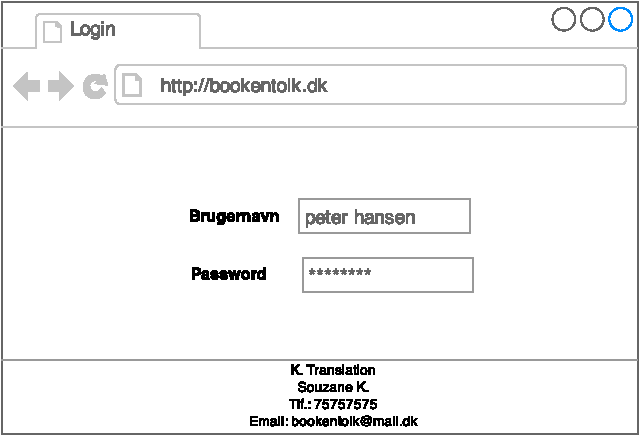
\includegraphics{mock1.pdf}
\caption{Mock-up tegning 1.}
\end{center}
\end{figure}


\newpage

\begin{figure}[!ht]
\begin{center}
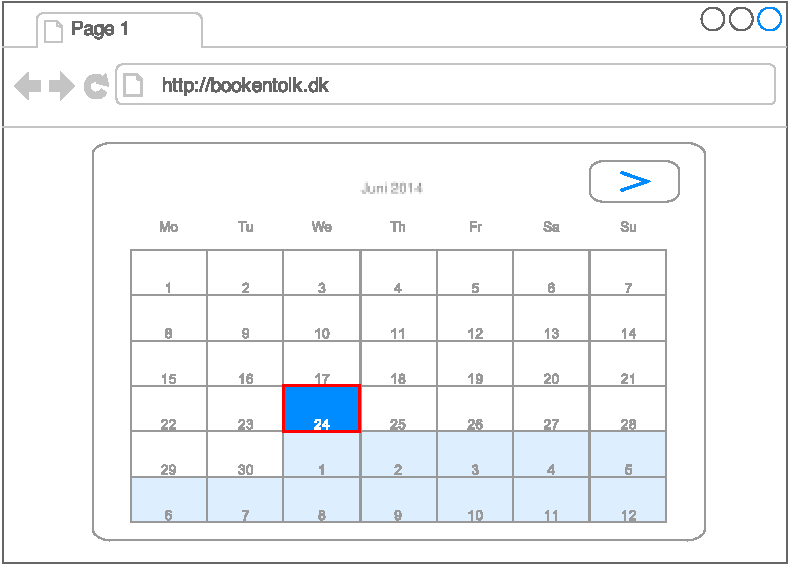
\includegraphics{mock2.pdf}
\caption{Mock-up tegning 2.}
\end{center}
\end{figure}


\newpage

\begin{figure}[!ht]
\begin{center}
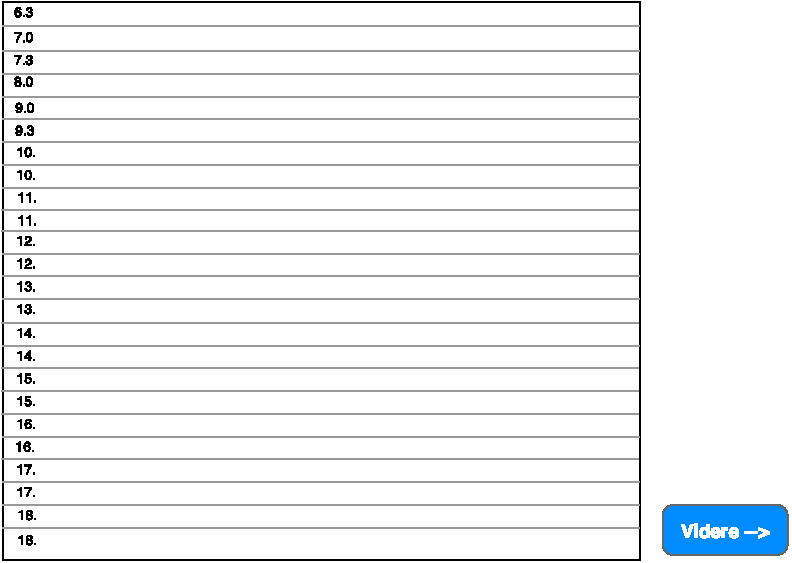
\includegraphics{mock3.pdf}
\caption{Mock-up tegning 3.}
\end{center}
\end{figure}


\newpage

\begin{figure}[!ht]
\begin{center}
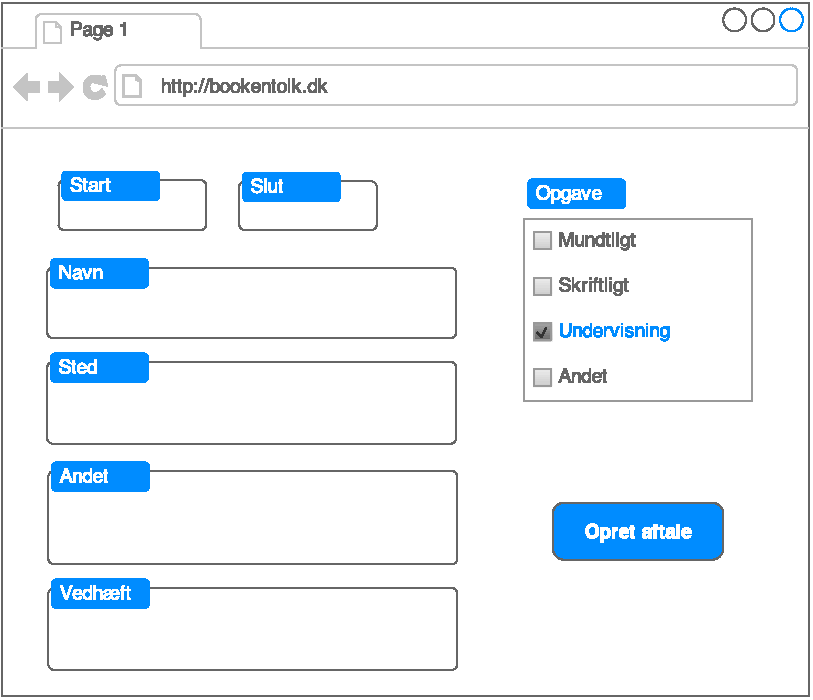
\includegraphics{mock4.pdf}
\caption{Mock-up tegning 4.}
\end{center}
\end{figure}


\newpage

\begin{figure}[!ht]
\begin{center}
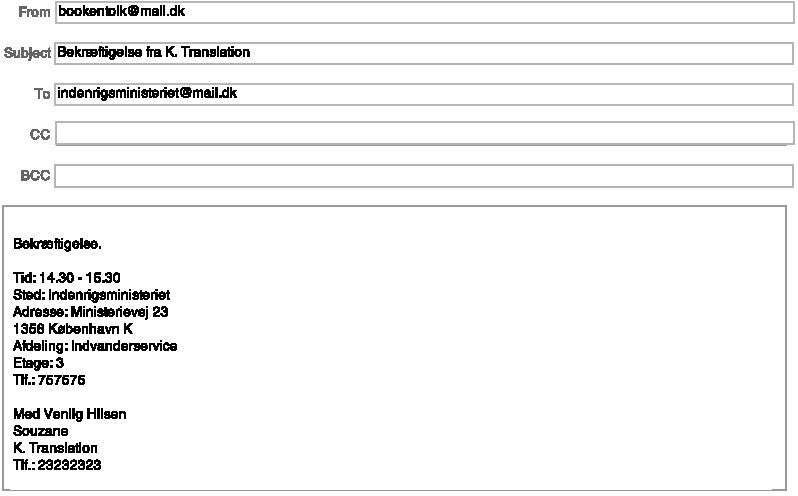
\includegraphics{mock5.pdf}
\caption{Mock-up tegning 5.}
\end{center}
\end{figure}

\newpage

\subsection{Bilag B: Første product- og sprint backlog}

\begin{center}
	\begin{tabular}{|p{8cm}|l|l|l|}
		\hline
Punkt & Prioritet & Værdi & Timer \\ \hline
Som bruger af KT's hjemmeside bliver man præsenteret for en kalender, hvori man
kan booke en aftale med KT. & 1 & Høj &  50 \\ \hline
Som KT's kunde møder man et login interface, når man navigerer til hjemmesiden. & 2 &
Høj & 15  \\ \hline
KT skal have muligheden for løbende at tilføje kunder til databasen. & 3 & Høj
& 15 \\ \hline
Man skal som kunde modtage en bekræftende email efter at have lavet en aftale
i kalenderen. KT skal ligeledes modtage en email med aftalen. & 4 & Middel & 10  \\ \hline
Som kunde bliver man præsenteret for en lille menu, hvor man skal vælge typen
på arbejdet. & 5 & Lav & 20\\ \hline
Som kunde skal man kunne søge i kalenderen ved hjælp af dato eller klokkeslet.
& 6  & Middel &  25 \\ \hline
Indehaveren af KT vil gerne kunne synkronisere sin eksterne kalender med
hjemmesidens kalender og på den måde overføre sine private aftale. & 7 & Lav &
 35 \\ \hline
KT ønsker en hjemmeside med kontaktinformation, billeder og et enkelt design.
& 8 & Middel & 12 \\ \hline
\end{tabular}
\end{center}
\begin{center}\textbf{Første Produkt Backlog}
\end{center}
\vspace{0.5cm}



\begin{center}
	\begin{tabular}{|l|p{4cm}|l|l|}
		\hline
		Backlog punkt & Sprint opgave & Frivillig & Timer\\ \hline
		\multirow{4}{4cm}{Som KT's kunde møder man et login interface,
		når man navigerer til hjemmesiden.} & Oprette en Django
		applikation & Omar  & 2 \\
		& Skriv login interfacet & Morten & 6 \\
		& Test login interfacet & Omar & 3 \\
		& Integrer interfacet med resten af hjemmesiden & Morten og Omar
		& 4 \\ \hline
		\multirow{3}{4cm}{KT ønsker en hjemmeside med
		kontaktinformation, billeder og et enkelt design.} &
		Skrive basisskabelonen til Django & Morten & 5 \\
		& Udvid basisskabelonen med Djangos ``extend''-skabeloner & Morten & 5
		\\ & Test hjemmesiden i flere forskellige browsere & Omar & 2 \\
		\hline

	\end{tabular}
\end{center}

\begin{center}
\textbf{Første Sprint Backlog}
\end{center}

\vspace{0.5cm}

\newpage



\subsection{Bilag C: Referater af kundemøder}

Kundereferat af 1. møde med K.Translation 

Det indledende møde fandt sted på kundens kontor på Østerbro. Kunden havde ved andre sammenhænge givet udtryk for frustrationer og ærgrelser over tabt arbejdsfortjeneste og usammenhængende tider og booking heraf. I denne forbindelse gjorde jeg kunden bekendt med vores  kommende projekt og tilbød vores assistance og stå til rådighed med denne udfordring. 

Det første møde var således kundes og vores ideface og brainstorm, hvor kunden bare frit skulle forklare hvordan disse frustrationer og udfordringer konkret former sig. Det var tydeligt for os som it-konsulenter, at kunden havde et it-behov og ved manglende kompetence var det oplagt at vi skulle hjælpe til og ligge en strategi for hvordan vi på bedst mulig vis kunne gennemføre et succesfuldt projekt. De første spørgsmål som indgik I mødet var således. Hvad er dine udfordringer og hvordan kommer de til udtryk? Hun forklarede at hendes udfordringer var at huske alle de aftaler der var indgået og at kunne bevare overblik over hvem og hvornår der var aftalt tidspunkt for hendes tolkeservicejobs. Derfor ville en mulig it-løsning aflaste de aftener med papir og alle de manuelle indtastninger hun foretog gang på gang.  Hvad tror du kan afhjælpe dine udfordringer.? It-system hvor det hele skulle køre igennem, var hvad hun anså som en problemløser for denne arbejdsmæssige udfordring. For også at kunne gøre det nemmere for hendes samarbejdspartner. Hvor mange samarbejdspartner sammen arbejder du med? Hertil svarede hun at hun havde advokater, politi og retssystemet og somme tide andre ínstitutioner hvor hendes opgave var at oversætte fra arabisk. Hvordan ønsker du systemet? Systemet skal være simpelt og nemt og let tilgængeligt for hende og hendes samarbejdspartnere. 

Vi kom frem til følgende punkter som vi ville arbejde videre på og som var I overensstemmelse med hvilke muligheder og hvilket kompetencer vi kunne tilbyde med dette projekt.  

Efterfølgende blev vi enige om at en konkretisering af hvilke parter som skulle have adgang til systemet og ikke mindst hvordan systemet skulle arbejde var noget vi aftalte vi skulle have på plads til næste møde. Konklusionen og det sidste KT ønskede var at booking systemet skulle være enkelt og ikke for kompliceret. 

\newpage

Referat af andet kundemøde.\\

Deltagere: Omar Khalidan, Souzanne Khalidan, Morten Trolle
Sted: Biocenter. Fredag den 9. maj 2014. Klokken 13 - 14.30.\\

Andet kundemøde startede med, at Souzanne gennemgik hvilke opgavetyper, hun som tolk oftest kommer ud for. Til det formål præsenterede hun os for en række mails og faxbeskeder, hvor hendes samarbejdspartnere havde booket hende til en opgave. I forhold til sidste kundemøde blev kundegrundlaget yderligere udspecificeret, idet hun detaljeret fortalte hvilke samarbejdspartnere, der bruger hende; hvor mange, der bruger hende; på hvilke tidspunkter, de bruger hende. I forhold til det første kundemøde, blev vi måske lidt overraskede over antallet af samarbejdspartnere, som hun anslog til omkring 100. Det blev også præciseret, at det ikke er den samme person hos hver partner, der booker Souzanne, men at der i politiet f.x. godt kan være flere forskellige, der booker hende. \\
I den forbindelse snakkede vi også om brugeroprettelse, og om Souzanne selv skal lægge sine kunder ind i systemet, eller om kunderne opretter sig selv. Vi blev enige om, at Souzanne oprettter de brugere, der er til systemet, da dette vil være det letteste for hendes kunder. Hun vil så præsentere dem for et brugernavn og password, så de efterfølgende kan logge på kalenderen. \\
Vi diskuterede også flere problemstillinger ved selve kalenderen. Souzanne vil gerne have, at brugerne i kalenderen kan se, om hun er optaget, og hvis hun er optaget, om det er fordi, hun slet ikke er til at træffe (f.x. ved ferie), eller om kunderne kan træffe hende telefonisk. Vi snakkede om at løse problemet med forskellige farvekoder for de forskellige aftaletyper, så booket kunne være grøn, ledig kunne være rød osv. \\
Når kunderne booker en tid, skal de også oplyse flere ting, såsom sted, adresse, afdeling, etage, forventet tid, opgavetype (mundtligt, skriftligt, telefonisk). 
Souzanne havde også i forhold til første kundemøde tænkt over, om hendes faktureringssystem på en eller anden måde kunne spille sammen med kalenderen og specielt alle aftalerne i kalenderen. Da hun arbejder meget og derfor har meget travlt, kan hun sagtens glemme at sende en faktura for udført arbejde. Hun ville gerne have denne proces automatiseret på en eller anden måde, og vi sagde, at vi ville undersøge dette uden dog at love hende noget. Evt. kan det være, at vi i sommerferien arbejder videre på systemet og får noget sådant implementeret. \\
Vi kom også ind på spørgsmålet om, hvor det endelige system skal placeres. Det vil være for dyr en løsning for Souzanne og K. Translation at købe en helt ny server til at hoste systemet på, så vi blev enige om, at Omar og jeg finder et webhotel eller en anden udbyder af serverplads. På den måde får Souzanne også så lidt med systemets daglige drift at gøre, og det er en stor prioritet for hende. Vi spurgte også ind til en ønsket hjemmesideadresse, og kom frem til noget i stil med (hvis den er ledig): bookentolk.dk.  
Til sidst snakkede vi også om præsentationen af hjemmesiden. Som det også fremgik på første kundemøde, skal det være så let for kunden som muligt at booke en tid. Derudover vil Souzanne gerne have hjemmesiden holdt i lyse pastelfarver evt. blandet med sort.

\newpage

Referat af tredie kundemøde.\\

Deltagere: Omar Khalidan, Souzanne Khalidan, Morten Trolle
Sted: Diku. Fredag den 30. maj 2014. Klokken 12 - 13.

Vi mødtes med Souzane for tredie gang for at gøre status og lave et kort review af projektet. Vi præsenterede hende for det arbejde, som vi havde lavet siden sidste møde, og hun kunne nu se flere af funktionere i brug. Hun prøvede også selv de funktioner, det var muligt på daværende tidspunkt. Vi forklarede hende så, hvordan vi havde planlagt at fortsætte projektet, og hvilke dele vi stadig manglede at implementere. \\
Souzane var ganske tilfreds med projekt og kalenderen, og vi diskuterede, hvor godt vi havde ramt hendes forventninger, og hvor projektet afviger fra kravspecifikationen. \\
Vi diskuterede også behovet for og besværgerligheden ved validering af bruger input. Alt bruger input skal valideres, og dette giver nogle udfordringer. F.eks. har vi valgt, at brugere  af kalenderen kun kan vælge imellem fastlagte tidspunktet (14.00, 14.30, 15.00, etc), eftersom dette betyder, at validering og håndtering af tidspunkter bliver en hel del lettere i forhold til, hvis brugere helt frit kunne vælge tidspunktet og ikke mindst formatet på tidspunktet. Der findes adskillige måder at skrive et klokkeslet på, men med på forhånd valgte klokkeslet undgår vi dette problem. Souzane var indforstået med denne løsning. \\ 
Vi forklarede hende også, at vi pt. er meget pressede på tid, og at det ikke er sikkert, at vi når helt i mål med hele projektet. Dette havde hun stor forståelse for, men vi understregede, at vi selvfølgelig gør alt, hvad vi kan for at færdiggøre projektet. Hun gjorde igen, ligesom sidste på sidste kundemøde, os opmærksomhed på behovet for en sådan kalender, vi er ved at udvikle, og mulighederne, der ligger i det, da mange af hendes tolke kollegaer står i samme situation som Souzane.  
\newpage

\subsection{Bilag D: Commit-log}

commit 79f162731bc52b893c52f0ea9547ff1236ac6da4
Author: morten trolle <morten.trolle@gmail.com>
Date:   Wed Jun 4 00:49:26 2014 +0200

    4 commit

commit 48c4f0d6297fac6179cd81f7d5ff0989901b42b6
Author: mhtn <morten.trolle@gmail.com>
Date:   Sun Jun 1 05:50:28 2014 +0200

    Update date.html

commit a7a1084a6bbbcefbca9103cb3f5fe1c7920094ab
Author: mhtn <morten.trolle@gmail.com>
Date:   Sun Jun 1 05:50:07 2014 +0200

    Update base2.html

commit dcee4b63d9e90067c75522efe4e7bd3707a8f5d3
Author: mhtn <morten.trolle@gmail.com>
Date:   Sun Jun 1 05:49:44 2014 +0200

    Update models.py

commit 9bb5fc8df8ab35c1372ef3246d2141390875194c
Merge: 3e40440 d1f58df
Author: morten trolle <morten.trolle@gmail.com>
Date:   Sun Jun 1 05:45:17 2014 +0200

    Merge branch 'master' of github.com:mhtn/tolkeservice

commit 3e4044020665a3d8dc853302c6941d35691b97cf
Author: morten trolle <morten.trolle@gmail.com>
Date:   Sun Jun 1 05:45:02 2014 +0200

    3 commit

commit d1f58dfc0a529807564ee68d3f82b8d9e420cab5
Author: okhalidan <khalidan@mac.com>
Date:   Sat May 31 21:48:07 2014 +0200

    hej

commit f31d9dfb7b9ac61a9bc49a0fd3e57955f34571f6
Author: okhalidan <khalidan@mac.com>
Date:   Sat May 31 21:38:39 2014 +0200

    hej

commit 3281e8da5a2d05cc2632a9102b0e1e88bab306dd
Author: okhalidan <khalidan@mac.com>
Date:   Sat May 31 09:35:57 2014 +0200

    hej

commit 008d5f7f8ce4bcb69e1d1f5cadf6672391425c46
Author: okhalidan <khalidan@mac.com>
Date:   Sat May 31 09:25:12 2014 +0200

    hej

commit a9a7d1b08b91cff310f68696184538dc45676ec0
Author: okhalidan <khalidan@mac.com>
Date:   Sat May 31 09:14:47 2014 +0200

    hej

commit 5d9709b6b14df09671428fea4161abe592b52974
Author: morten trolle <morten.trolle@gmail.com>
Date:   Fri May 30 01:39:27 2014 +0200

    3. commit

commit b8c29a71dc3aa2b944baedbf7eea5049ca400ce1
Author: okhalidan <khalidan@mac.com>
Date:   Wed May 28 13:34:01 2014 +0200

    hej

commit 8177788c1b509887de7a8f8b6fb8dcf69c9db799
Author: okhalidan <khalidan@mac.com>
Date:   Mon May 26 09:37:50 2014 +0200

    hej

commit f79ed6e00a06c0733cbde3d1c7c09ae313410c55
Author: okhalidan <khalidan@mac.com>
Date:   Mon May 26 09:36:59 2014 +0200

    hej

commit 8ccd1f797909fec69f9dbf1e384252af954e5454
Author: okhalidan <khalidan@mac.com>
Date:   Mon May 26 09:35:31 2014 +0200

    hej

commit f9b377e2d78e0fbf843dbbd4d8131c166f3c814b
Author: okhalidan <khalidan@mac.com>
Date:   Mon May 26 09:34:17 2014 +0200

    he

commit 4a1d92faa38545f811c40299e1ed13a18a1dab2e
Author: okhalidan <khalidan@mac.com>
Date:   Mon May 26 09:33:15 2014 +0200

    hej

commit ec5a23ca5640f1a7abedba00e242d6e00ad3a666
Author: okhalidan <khalidan@mac.com>
Date:   Thu May 22 14:27:14 2014 +0200

    hej

commit cca20d896b0f38a44cc1b1c1d06756146adcbf1e
Author: okhalidan <khalidan@mac.com>
Date:   Thu May 22 11:21:01 2014 +0200

    hej

commit bc2102277a7d4022237db88ee3d4200f2bb4495b
Author: okhalidan <khalidan@mac.com>
Date:   Thu May 22 11:19:56 2014 +0200

    hej

commit 61d3fd30989db4ba68faafcad733b43cec82b0c5
Author: okhalidan <khalidan@mac.com>
Date:   Thu May 22 11:19:03 2014 +0200

    hej

commit 6b248441dd842464c6b811fb92ffbfd5b2e04b6c
Author: okhalidan <khalidan@mac.com>
Date:   Thu May 22 11:17:56 2014 +0200

    hej

commit 3b6e7709d402dede77b614cb1773b8c36fa409ce
Author: okhalidan <khalidan@mac.com>
Date:   Thu May 22 11:17:07 2014 +0200

    hej

commit 40638db9443b3fcb6d08f3a7734406c3edc78a3b
Author: okhalidan <khalidan@mac.com>
Date:   Thu May 22 09:29:21 2014 +0200

    hej

commit 2ef27d916315113f0dba6a110674168217ad076e
Author: okhalidan <khalidan@mac.com>
Date:   Thu May 22 09:25:47 2014 +0200

    hej

commit ab088d022a46668d591ab2fe30251cc14ef4e952
Author: okhalidan <khalidan@mac.com>
Date:   Wed May 21 16:58:54 2014 +0200

    hej5

commit f7ddd15deece6052cce2667a722c6dd5c68788d6
Author: okhalidan <khalidan@mac.com>
Date:   Wed May 21 16:58:03 2014 +0200

    hej4

commit 7d7aa119472d4c5f718df5f1541260ace7f24ba8
Author: okhalidan <khalidan@mac.com>
Date:   Wed May 21 16:57:37 2014 +0200

    hej

commit 0a0cdd240d17b230c1e5a01687d04c8eeb6944c5
Author: okhalidan <khalidan@mac.com>
Date:   Wed May 21 16:57:23 2014 +0200

    hej2

commit 277391b9ceaa546479c879ecbbdc8326286f28e5
Author: okhalidan <khalidan@mac.com>
Date:   Wed May 21 16:55:27 2014 +0200

    hej

commit c15a67f892416fd601794f8ab59a3f2142658c6e
Author: okhalidan <khalidan@mac.com>
Date:   Wed May 21 16:07:32 2014 +0200

    hej5

commit 5275e1f599f6d0740c3d71b725b3bbd6eb897e85
Author: okhalidan <khalidan@mac.com>
Date:   Wed May 21 16:07:02 2014 +0200

    hej4

commit 5ea33b5f8bf2477f176a7139ac240dd90ef1bd75
Author: okhalidan <khalidan@mac.com>
Date:   Wed May 21 16:06:28 2014 +0200

    hej3

commit 17e6823c3791f48a828fc9a8d398095336768cca
Author: okhalidan <khalidan@mac.com>
Date:   Wed May 21 16:06:11 2014 +0200

    hej2

commit ee7ad36b717f34274b5b788adf930f5832bc27d7
Author: okhalidan <khalidan@mac.com>
Date:   Wed May 21 16:05:54 2014 +0200

    hej

commit 7cec0fc4a29ed50954e54823ead4a410aac4d009
Author: okhalidan <khalidan@mac.com>
Date:   Tue May 20 13:54:12 2014 +0200

    hej morten

commit d87ab37ae2fb16b610fbf3cb639d3764df03f941
Author: okhalidan <khalidan@mac.com>
Date:   Mon May 19 09:20:27 2014 +0200

    hej morten

commit 74f106b166f9c55adaafb173d2cfede2e3c979f7
Author: okhalidan <khalidan@mac.com>
Date:   Mon May 19 09:20:04 2014 +0200

    hej morten

commit 77cbce888eb34a17b136f9f9d6de99076d939fcf
Author: okhalidan <khalidan@mac.com>
Date:   Mon May 19 09:19:41 2014 +0200

    hej morten

commit be375c414d04677f470e605f0d89abb1d1169696
Author: okhalidan <khalidan@mac.com>
Date:   Mon May 19 09:19:22 2014 +0200

    hej morten

commit 9868bc02c6a292eb301c5eb1f174bbb5ce10af72
Author: okhalidan <khalidan@mac.com>
Date:   Mon May 19 09:18:56 2014 +0200

    hej morten

commit ccc9678f0c9bcf6e552281eb5ca20a4d44ba28bd
Author: okhalidan <khalidan@mac.com>
Date:   Mon May 19 09:18:03 2014 +0200

    hej morten

commit ab8a8672186f3ce214e318fd1c1d8563cf1a4723
Author: mhtn <morten.trolle@gmail.com>
Date:   Sun May 18 22:34:45 2014 +0200

    Update README.md

commit 1e4789144f59b180643fb4934e091a447ed1512b
Author: mhtn <morten.trolle@gmail.com>
Date:   Sun May 18 22:34:31 2014 +0200

    Update README.md

commit 00c7703971aa3ce3b6b2c4037e456daf8208dfc3
Author: mhtn <morten.trolle@gmail.com>
Date:   Sun May 18 22:32:48 2014 +0200

    Update andenrapport.tex

commit 01d04d3d31c215e17b0c216fbca13a2fc8541cd7
Author: mhtn <morten.trolle@gmail.com>
Date:   Sun May 18 22:32:29 2014 +0200

    Update andenrapport.tex

commit 7b00cda0810b4ac9fa97113b8edc3e976e4de6a2
Author: okhalidan <khalidan@mac.com>
Date:   Thu May 15 15:32:54 2014 +0200

    hej

commit 6d651c8a6f320b7126e5e6f3ca3843aeeae493d5
Author: okhalidan <khalidan@mac.com>
Date:   Thu May 15 15:30:42 2014 +0200

    Omar redigering

commit f4220417267bfba80297ded4c8a1116fb8bdee0e
Author: okhalidan <khalidan@mac.com>
Date:   Thu May 15 15:24:13 2014 +0200

    Omar Redigering

commit 9a5f4ce370aa5c1ba0f07c15db6dc947c9a3d19e
Author: okhalidan <khalidan@mac.com>
Date:   Thu May 15 15:21:12 2014 +0200

    Omar Redigering

commit d6115f2e83301d1baa851f102c755d01748d6a40
Author: okhalidan <khalidan@mac.com>
Date:   Thu May 15 15:19:21 2014 +0200

    Omar redigering

commit 0a67f94aea03b3a6870bdf01505b737e38a75e0d
Author: okhalidan <khalidan@mac.com>
Date:   Thu May 15 15:17:42 2014 +0200

    Omar redigering

commit 0fde5007086efb818edd8694135867d19b41f06c
Author: okhalidan <khalidan@mac.com>
Date:   Thu May 15 15:07:27 2014 +0200

    Omar redigering

commit ab5d2c7027dd06f80d0fd3cbae71a61b84d2e159
Author: okhalidan <khalidan@mac.com>
Date:   Thu May 15 09:51:14 2014 +0200

    hej

commit c2a340223c51edd0413018fa64db0da31273b33e
Author: okhalidan <khalidan@mac.com>
Date:   Thu May 15 09:48:17 2014 +0200

    hejmeddig

commit 449194f3b77521b813dc8f336d7f24b2839a2c81
Author: okhalidan <khalidan@mac.com>
Date:   Thu May 15 09:40:44 2014 +0200

    hej dalal

commit 87f9aff90c436cef8ddffd0572c0a146534ad146
Author: okhalidan <khalidan@mac.com>
Date:   Thu May 15 09:14:22 2014 +0200

    hej morten

commit 7dbb939519165696a448554516442196e8fce778
Author: okhalidan <khalidan@mac.com>
Date:   Thu May 15 08:58:29 2014 +0200

    hej

commit 3a7e9c2d12034f026630573ef8896b162830fab6
Merge: 8b37e11 84f5d83
Author: okhalidan <khalidan@mac.com>
Date:   Thu May 15 08:51:46 2014 +0200

    Merge branch 'master' of github.com:mhtn/tolkeservice

commit 8b37e11cbca4b162f45c62d2c98bcea0b700419b
Author: okhalidan <khalidan@mac.com>
Date:   Thu May 15 08:51:29 2014 +0200

    hej med dig

commit 84f5d836e448d8846f4530a5de66c1687257e155
Author: morten trolle <morten.trolle@gmail.com>
Date:   Wed May 14 22:59:09 2014 +0200

    commit

commit 9a39166a5c0a9ac94efae2e141bc6eb87076b884
Author: morten trolle <morten.trolle@gmail.com>
Date:   Wed May 14 21:10:30 2014 +0200

    commit

commit feb32b52a92e6d72959aee72777c10baaf3a6a38
Author: okhalidan <khalidan@mac.com>
Date:   Wed May 14 14:14:20 2014 +0200

    hej morten

commit 5ba0cfc2310bac316a4e38cca1a27dbf0777e1ed
Author: morten trolle <morten.trolle@gmail.com>
Date:   Wed May 14 14:08:30 2014 +0200

    commit

commit f43793a45e2ddee9a767321e4b91a4c8c51efa1c
Author: okhalidan <khalidan@mac.com>
Date:   Wed May 14 12:32:47 2014 +0200

    hej morten - dette er bare en test -m

commit 4b0bcb809acde7f2c0ec36f983ebffaea4db1de3
Author: okhalidan <khalidan@mac.com>
Date:   Wed May 14 10:16:51 2014 +0200

    Update tests.py
    
    omar test1

commit 5beeaaed5755a82135e1c75f7f0ac39eca925e23
Author: mhtn <morten.trolle@gmail.com>
Date:   Wed May 14 00:47:48 2014 +0200

    Update andenrapport.tex

commit d5ad5061c5dbcedde0219d6acb10ec877214e528
Merge: 80fac68 1492984
Author: morten trolle <morten.trolle@gmail.com>
Date:   Wed May 14 00:45:30 2014 +0200

    Merge branch 'master' of github.com:mhtn/tolkeservice

commit 80fac683de92d7f8f8e0a0d3c2bf561ee5f4f3df
Author: morten trolle <morten.trolle@gmail.com>
Date:   Wed May 14 00:45:12 2014 +0200

    commit

commit 149298416f0219536f3a646c8b1a70e65ab64215
Author: okhalidan <khalidan@mac.com>
Date:   Tue May 13 14:16:12 2014 +0200

    Update andenrapport.tex

commit 90c005eb8955a9f3e919640b29ddb88d6029bbbf
Author: okhalidan <khalidan@mac.com>
Date:   Tue May 13 13:12:07 2014 +0200

    Update andenrapport.tex

commit bf65fcfbb60064731fec1a4b2f7d83bb3027f048
Author: okhalidan <khalidan@mac.com>
Date:   Tue May 13 13:11:48 2014 +0200

    Update andenrapport.tex

commit 4e4f9d128035c7a50f0b74d34130f07a66775198
Author: mhtn <morten.trolle@gmail.com>
Date:   Sun May 11 21:20:22 2014 +0200

    Update andenrapport.tex

commit 3296da5b7f2ce57c4df3f72c4833fe65223ee564
Author: mhtn <morten.trolle@gmail.com>
Date:   Sun May 11 21:20:05 2014 +0200

    Update andenrapport.tex

commit 46c13583514134a7cd1b219a0c2a212ea016d107
Author: mhtn <morten.trolle@gmail.com>
Date:   Sun May 11 21:19:05 2014 +0200

    Update andenrapport.tex

commit a2c933c6656a27e88b4a5c6dd53b965df5e542b5
Author: mhtn <morten.trolle@gmail.com>
Date:   Sun May 11 21:18:44 2014 +0200

    Update andenrapport.tex

commit 4bf17fbae5b2ed475630de40779612beb655d496
Author: morten trolle <morten.trolle@gmail.com>
Date:   Sun May 11 21:17:57 2014 +0200

    commit

commit cc931efb469780f5b637ff07ebeca835b578d388
Author: mhtn <morten.trolle@gmail.com>
Date:   Sat May 10 22:35:02 2014 +0200

    Update andenrapport.tex

commit ddfb72b523101ef1f10d2aa7f0394ecbe42eb678
Author: mhtn <morten.trolle@gmail.com>
Date:   Sat May 10 22:34:32 2014 +0200

    Update andenrapport.tex

commit a264f1c4418a17f57b54e2867b470e8cb610612b
Author: mhtn <morten.trolle@gmail.com>
Date:   Sat May 10 22:32:43 2014 +0200

    Update andenrapport.tex

commit f52c5c441d8d584756069c81d52d9f309cc38eeb
Author: mhtn <morten.trolle@gmail.com>
Date:   Sat May 10 22:31:01 2014 +0200

    Update andenrapport.tex

commit 8f0e79198e525a12a1d4a6b4c44f605e5b7cc531
Author: mhtn <morten.trolle@gmail.com>
Date:   Sat May 10 22:30:05 2014 +0200

    Update base2.html

commit 0a66940249f366499e543259f136ea564648e41a
Author: morten trolle <morten.trolle@gmail.com>
Date:   Sat May 10 22:14:49 2014 +0200

    commit

commit 886db9ef288a3d1e29236e7fde14e8e4364bf13e
Author: morten trolle <morten.trolle@gmail.com>
Date:   Fri May 9 12:31:49 2014 +0200

    django-kode

commit cbadc056147c1fcbff4cb09e2aae0fb492c04092
Merge: da44388 533739c
Author: morten trolle <morten.trolle@gmail.com>
Date:   Thu Apr 24 01:58:32 2014 +0200

    Merge branch 'master' of github.com:mhtn/tolkeservice
    
    Conflicts:
    	andenrapport.aux
    	andenrapport.log
    	andenrapport.toc

commit da4438868291b77b11dc6ac7845db93ce550d7f8
Author: morten trolle <morten.trolle@gmail.com>
Date:   Thu Apr 24 01:54:36 2014 +0200

    anden rapport

commit 533739c32c0689495c8b8359b1f8d8c02a8032ab
Author: mhtn <morten.trolle@gmail.com>
Date:   Mon Apr 21 23:56:19 2014 +0200

    Delete andenrapport.log

commit 72ac72c54c56b7ca91225b06a0b9c57779929bb2
Author: mhtn <morten.trolle@gmail.com>
Date:   Mon Apr 21 23:56:01 2014 +0200

    Delete andenrapport.toc

commit 21eb8f9154fb5b12ad09ee3839beb63d72ea5396
Author: mhtn <morten.trolle@gmail.com>
Date:   Mon Apr 21 23:55:51 2014 +0200

    Delete andenrapport.aux

commit 2b0acff80dbc7cc51493ca13532fd4d8bfb0362c
Author: morten trolle <morten.trolle@gmail.com>
Date:   Mon Apr 21 23:54:13 2014 +0200

    anden rapport

commit c7864f490e0986d67247cea2848a0e19b2bf7b3f
Author: morten trolle <morten.trolle@gmail.com>
Date:   Sat Apr 19 03:33:46 2014 +0200

    anden rapport

commit e35594a89cc68cf5d91f0153f88ba431ec7da4f0
Author: morten trolle <morten.trolle@gmail.com>
Date:   Wed Apr 16 02:12:40 2014 +0200

    initial commit

commit b87f59d9036d9591c3f39fc91699650f3001e55c
Author: mhtn <morten.trolle@gmail.com>
Date:   Mon Apr 14 04:22:03 2014 -0700

    Initial commit


\end{document}











